\documentclass[12pt]{article}

\usepackage{fullpage}
\usepackage{breqn}
\usepackage{epsfig}
\usepackage{longtable}
\usepackage{fontenc}
\usepackage{graphicx}
\usepackage{times}
\usepackage{rotating}
\usepackage{psfrag}
\usepackage{graphics}
\usepackage{lscape}
\usepackage{xspace}
\usepackage{hyperref}


\bibliographystyle{input/prsty}

\input{input/0_defs.tex}

%%%%%%%%%%%%%%%

\begin{document}

\pagestyle{empty}
 
%\begin{center}
% \LARGE{
%  Tensor Asymmetry $A_{zz}$ in the $x>1$ Region
% }
%\end{center}
%
%\hrule \vspace{.05cm}\hrule
%
%\input{input/0_author.tex}

%\newpage

%\begin{abstract}
%  \input{input/0_abstract.tex}
%\end{abstract}

\newpage

%\section*{Foreword}

%This proposal is an update to PR12-11-110 which was submitted to PAC38.  For convenience, we reproduce the PAC report on the next page.   We provide here an overview of the actions we've taken to address the PAC concerns. Full details are available in the main text.

As suggested by PAC38, we have modified our experimental technique to measure the tensor asymmetry instead of the cross section difference.  This takes the simplified form of the ratio of tensor polarized to unpolarized cross-sections shown in Eq.~\ref{3}.   While this cancels the largest first order effects\footnote{For example, the target magnetic field will be oriented along the beamline during both polarized and unpolarized data taking, which greatly reduces the sensitivity to changes in acceptance in the two configurations.}, special care will be needed to control the sensitivity of the integrated counts in each state to time dependent drifts in detector response, charge measurement and luminosity. 

We have assumed a tensor polarization (P$_{zz}$=\PZZ\%) which is larger than the previous proposal. This assumption is based on the documentation of tensor polarized targets previously discussed in publications, and is supported by the experience of the collaboration's polarized target groups.   This will require incremental development of existing DNP techniques.  We acknowledge that less established methods, such as the `hole-burning' technique recommended by the PAC, hold very good potential to produce significantly higher tensor polarization, but this will require significant R\&D.  We have initiated this process, although from a practical perspective, the funding for this development will likely remain limited until an approved experiment demonstrates the need for these novel tensor polarized targets. 

The $x_B$-coverage has been expanded, although we note that a significantly non-zero value of $b_1$ at any $x_B$ would unambiguously confirm its non-conventional behavior.  Finally, we have engaged several theorists for calculations and to confirm that our interpretation of the relationship between the measured asymmetry and the tensor structure function $b_1$ is valid.



\newpage
\subsection*{PAC38 Report}
{
\noindent
{\bf PR12-11-110} ``The Deuteron Tensor Structure Function b1''

\vspace{0.1cm}
\noindent
{\bf Motivation}: This proposal, a follow-up of LOI-11-003 submitted to PAC37, is dedicated to the measurement of the deuteron tensor structure function $b_1$ by measuring deep inelastic scattering from a tensor polarized deuterium target. All available models predict a small or vanishing value of $b_1$ at low x, however the first pioneering measurement of $b_1$ at HERMES revealed a crossover to an anomalously large negative value, albeit with a relatively large experimental uncertainty. This justifies the intention to make a precise measurement: confirmation that $b_1$ is relatively large may then require an explanation based on more exotic models for the deuteron, such as hidden color due to a 6-quark configuration.

%\vspace{1cm}
\noindent
{\bf Measurement and Feasibility}: The collaboration proposes to carry out this experiment in Hall C, using the polarized UVa/JLab ND$_3$ target, the HMS/SHMS spectrometers and an unpolarized 115 nA electron beam. The tensor structure function $b_1$ is derived from the measurement of the difference between the transversely and longitudinally tensor polarized cross-sections, which is directly proportional to $b_1$ itself. From the measured value of $b_1$ the tensor asymmetry $A_{zz}$ can be calculated, provided the structure function $F_1$ is known. The collaboration proposes to perform the measurement in 28 days of data taking at 11 GeV at the two x values of 0.3 and 0.5, which cover the range in which the HERMES data display the crossover of $b_1$ to large negative values.



%\vspace{1cm}
\noindent
{\bf Issues}: Despite the interesting physics case presented, the PAC has identified several issues with this proposal.
\begin{enumerate}
\item One obvious problem is the theoretical interpretation of the results of this kind of experiments. Following the recommendation of PAC37 the collaboration has partially addressed this question by expanding the discussion of the expected behavior of $b_1(x)$ in various theoretical models. However to draw significant conclusions from this measurement, also given the limited kinematical coverage (see below) chosen, would require further work.
\item The chosen x range, although overlapping with the region in which the HERMES results were obtained, does not seem sufficient to determine $b_1(x)$ in such a way as to unambiguously establish its conventional or exotic behavior. The PAC encourages the collaboration to explore the possibility to carry out the measurement using a large acceptance spectrometer covering a wider x range.
\item The PAC has concerns about the proposed experimental method using the cross section difference between the transversely and longitudinally tensor polarized target configurations. Given a 5-tesla field for this type of target, the effect on the acceptance due to the target field for these configurations can be quite different, and such systematic uncertainties due to the acceptance and other effects may well be larger than the effect that the proponents are trying to measure.
\item The proponents should pursue the tensor asymmetry measurement technique. Currently, the proposed target has a rather low tensor polarization ($\sim$10\%). It is crucial and important to pursue more vigorously techniques such as the RF ``hole’’ burning technique to improve the tensor polarization of the target.
%}
\end{enumerate}
}




\clearpage


\tableofcontents


\pagestyle{plain}

\clearpage

%\section{Quotes (To be removed)}
%\input{input/0_quotes.tex}

%\section{Background and Motivation}
%\input{input/1_intro.tex}
% \subsection{Tensor Structure of the Deuteron}
% \input{input/1_tensor_pol.tex}
% \subsection{Quasi-Elastic and $x>1$ Scattering from Spin-1 Targets}
% \input{input/1_b1_background.tex}

%\subsubsection{First Measurement of $b_1(x)$ by the HERMES Collaboration}
% \input{input/data.tex}

% \subsection{The Tensor Asymmetry \Azz}
%\label{PREDB1X}
%   \input{input/1_th_predictions.tex}


\section{The Proposed Experiment}

We propose to measure the tensor asymmetry $A_{zz}$ and tensor analyzing power $T_{20}$ from inclusive electron scattering from polarized deuterons in the quasi-elastic and elastic region of $\XMIN<x<\XMAX$, $\QMIN$~(GeV/$c)^2 < Q^2 <\QMAX$~(GeV/$c)^2$, and $\WMIN < W_{NN} < \WMAX$~GeV using the Hall C HMS and SHMS spectrometers at forward angle from a solid polarized ND$_3$ target.


\subsection{$A_{zz}$ Experimental Method} %Measurement of $A_{zz}$ }

The measured double differential cross section for electron scattering from a spin-1 target is characterized by a vector polarization $P_{z}$ and tensor polarization $P_{zz}$. With an unpolarized beam and the target field oriented along the beam, the cross section is expressed as~\cite{Leidemann:1991qs}
\begin{equation}
\frac{d^2\sigma_p}{d\Omega dE'}=\frac{d^2\sigma_u}{d\Omega dE'}\left(1+\frac{1}{2}P_{zz}A_{zz}) \right),
\label{eq:one}
\end{equation}
where $\sigma_p$ ($\sigma_u$) is the polarized (unpolarized) cross section and $A_{zz}$ is the
tensor asymmetry of the virtual-photon deuteron cross section.  This allows us to write
the polarized tensor asymmetry with positive tensor polarization using an unpolarized electron beam as
\begin{eqnarray}
\label{Azz}
A_{zz} = \frac{2}{P_{zz}}\left(\frac{\sigma_p - \sigma_u}{\sigma_u}\right).
\end{eqnarray}
The tensor polarization is given by 
\begin{equation}
P_{zz}=(p_++p_-)-2p_0,
\end{equation}
where $p_m$ represents the population in the $m_J=+1$,~$-1$,~or $0$ state.

Eq. \ref{Azz} reveals that the asymmetry $A_{zz}$ compares two different cross sections measured under different polarization conditions of the target: positively tensor polarized and unpolarized.  
To obtain the relative cross section measurement in the same configuration, the same target cup and material will be used at alternating polarization states (polarized vs. unpolarized),  and the magnetic field providing the quantization axis will be oriented along the beamline at all times.
This field will always be held at the same value, regardless of the target material polarization state. 
This process, identical to that used for the already-approved $b_1$ measurement~\cite{b1prop}, ensures that the acceptance remains consistent within the stability of the super conducting magnet.  


Since many of the factors involved in the cross sections cancel in
the ratio, Eq. \ref{Azz} can be expressed in terms 
of the charge normalized, efficiency corrected numbers of tensor polarized ($N_p$) and unpolarized ($N_u$) counts, 
\begin{eqnarray} \label{3}
A_{zz}&=&\frac{2}{fP_{zz}}\left(\frac{N_p - N_u}{N_u}\right) .
\end{eqnarray}

The dilution factor $f$ corrects for the presence of unpolarized nuclei in the target and is defined by
\begin{equation}
f=\frac{N_D\sigma_D}{N_N\sigma_N+N_D\sigma_D+\sum\limits_{A} N_A\sigma_A},
\end{equation}
where $N_D$ is the number of deuterium nuclei in the target and $\sigma_D$ is the corresponding inclusive double differential scattering cross 
section, $N_N$ is the nitrogen number of scattered nuclei with cross section $\sigma_N$, and $N_A$ is the number of other scattering nuclei of mass number $A$ with cross section $\sigma_A$. As has been noted in previous work~\cite{Frankfurt:1988nt}, the dilution factor at high $x$ drops off considerably until the SRC plateau region, as shown in Fig.~\ref{fdil}. By using a high-luminosity solid target at a small scattering angle $\theta_{e'}$, this effect will be counteracted. The dilution factor is a much smaller problem for elastic deuteron scattering at $x=2$.

\begin{figure}
\begin{center}
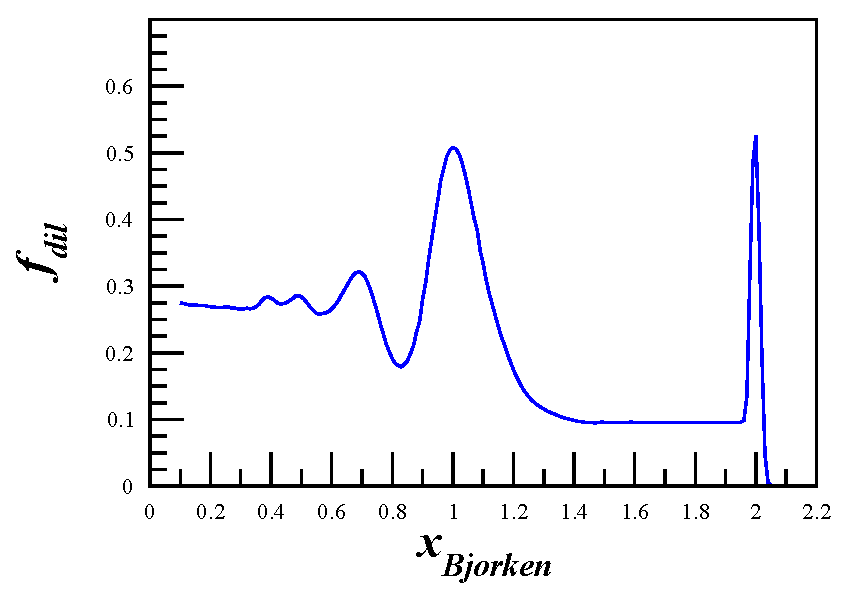
\includegraphics[width=0.45\textwidth]{figs/fdil_q2_15.eps}
\caption{\label{fdil}The estimated dilution factor, in this case at $Q^2=1.5 \mathrm{~(GeV}/c)^2$, is expected to drop off at high $x$ until it reaches the SRC plateau region and then the elastic peak at $x=2$. The low dilution factor of $1.1<x<1.95$ will be counteracted by using a high-luminosity target.}
\end{center}
\end{figure}

The dilution factor can be written in terms of the relative volume ratio of ND$_3$ to LHe in the target cell, otherwise known as the packing fraction $p_f$.  
In our case of a cylindrical target cell oriented along the magnetic field,the packing fraction is exactly equivalent to the percentage of the cell length filled with ND$_3$.  
%The dilution factor is discussed in further detail in Sec. \ref{dil}.

If the time is evenly split between scattering off of polarized and unpolarized ND$_3$, the time necessary to achieve the desired precision $\delta A$ is:
\begin{equation}
t=\frac{N_p}{R_p}+\frac{N_u}{R_u}=\frac{8}{f^2P_{zz}^2}\left(\frac{R_p(R_u+R_p)}{R_u^3}\right)\frac{1}{\delta A_{zz}^2}
\end{equation} 
where $R_{p(u)}$ is the polarized (unpolarized) rate and $N_{p(u)}$ is the total estimated 
number of polarized (unpolarized) counts to achieve the uncertainty $\delta A_{zz}$.  

%See Sec.~\ref{stat} for full details of the statistical uncertainty.


\subsection{Kinematics}
\label{kinematics}

\label{EXP}
We propose to measure the tensor asymmetry $A_{zz}$ for $\XMIN<x<\XMAX$, $\QMIN$~(GeV/$c)^2 < Q^2 <\QMAX$~(GeV/$c)^2$, and $\WMIN < W_{NN} < \WMAX$~GeV and extract the tensor analyzing power $T_{20}$ for $\QMINT20$~(GeV/$c)^2 < Q^2 <\QMAXT20$~(GeV/$c)^2$. Central kinematics of the spectrometers are given in Table~\ref{RATES1}
%, estimates for the uncertainties of $A_{zz}$ are given in Tables~\ref{RATES2}-\ref{RATES3}, and estimates for the uncertainties of $T_{20}$ are given in Table\need
. Fig.~\ref{kincov} shows the planned kinematic coverage utilizing the Hall C HMS and SHMS spectrometers at forward angles. 

\begin{table}
\begin{center}
\begin{tabular}{cc|c|c|c|c|c|c}
 & & $E_0$ & $Q^2$    	& $E'$  &    $\theta_{e'}$  &  Rates   & PAC Time   \\
%& (GeV) & (GeV$^2$)  & (GeV)  &     (deg.)   &   (kHz)  & (hours) \\
& & (GeV) & (GeV$^2$)  & (GeV)  &     ($^{\circ}$)   &   (kHz)  & (Days) \\
%\multicolumn{2}{|c|}{$\times 10^{-2}$}
\hline\hline
SHMS & (S1) & 8.8	&  1.5	&  8.36	&    8.2  	&    0.38	&   25 \\
HMS  & (H1) & 8.8	&  2.9	&  7.26	&    12.2	&    0.04	&   25 \\  
SHMS & (S2) & 6.6	&  0.7	&  6.35	&    7.5 	&    3.57	&   8 \\
HMS  & (H2) & 6.6	&  1.8	&  5.96	&    12.3	&    0.09	&   8 \\  
SHMS & (S3) & 2.2	&  0.2	&  2.15	&    10.9 	&    10.5	&   1 \\
HMS  & (H3) & 2.2	&  0.3	&  2.11	&    14.9	&    3.23	&   1 \\  
\hline\hline
\end{tabular}
\caption{\label{RATES1}Summary of the central kinematics and physics rates using the Hall C  spectrometers.}
\end{center}
\end{table}









\begin{figure}
\begin{center}
%\includegraphics[width=\textwidth]{figs/Pzz_30_all_q2_w.eps}
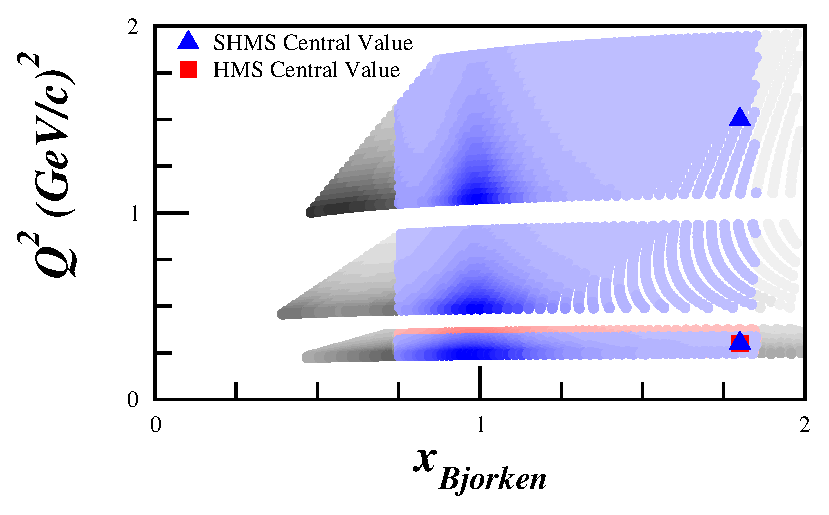
\includegraphics[width=0.49\textwidth]{figs/Pzz_30_all_q2.eps}

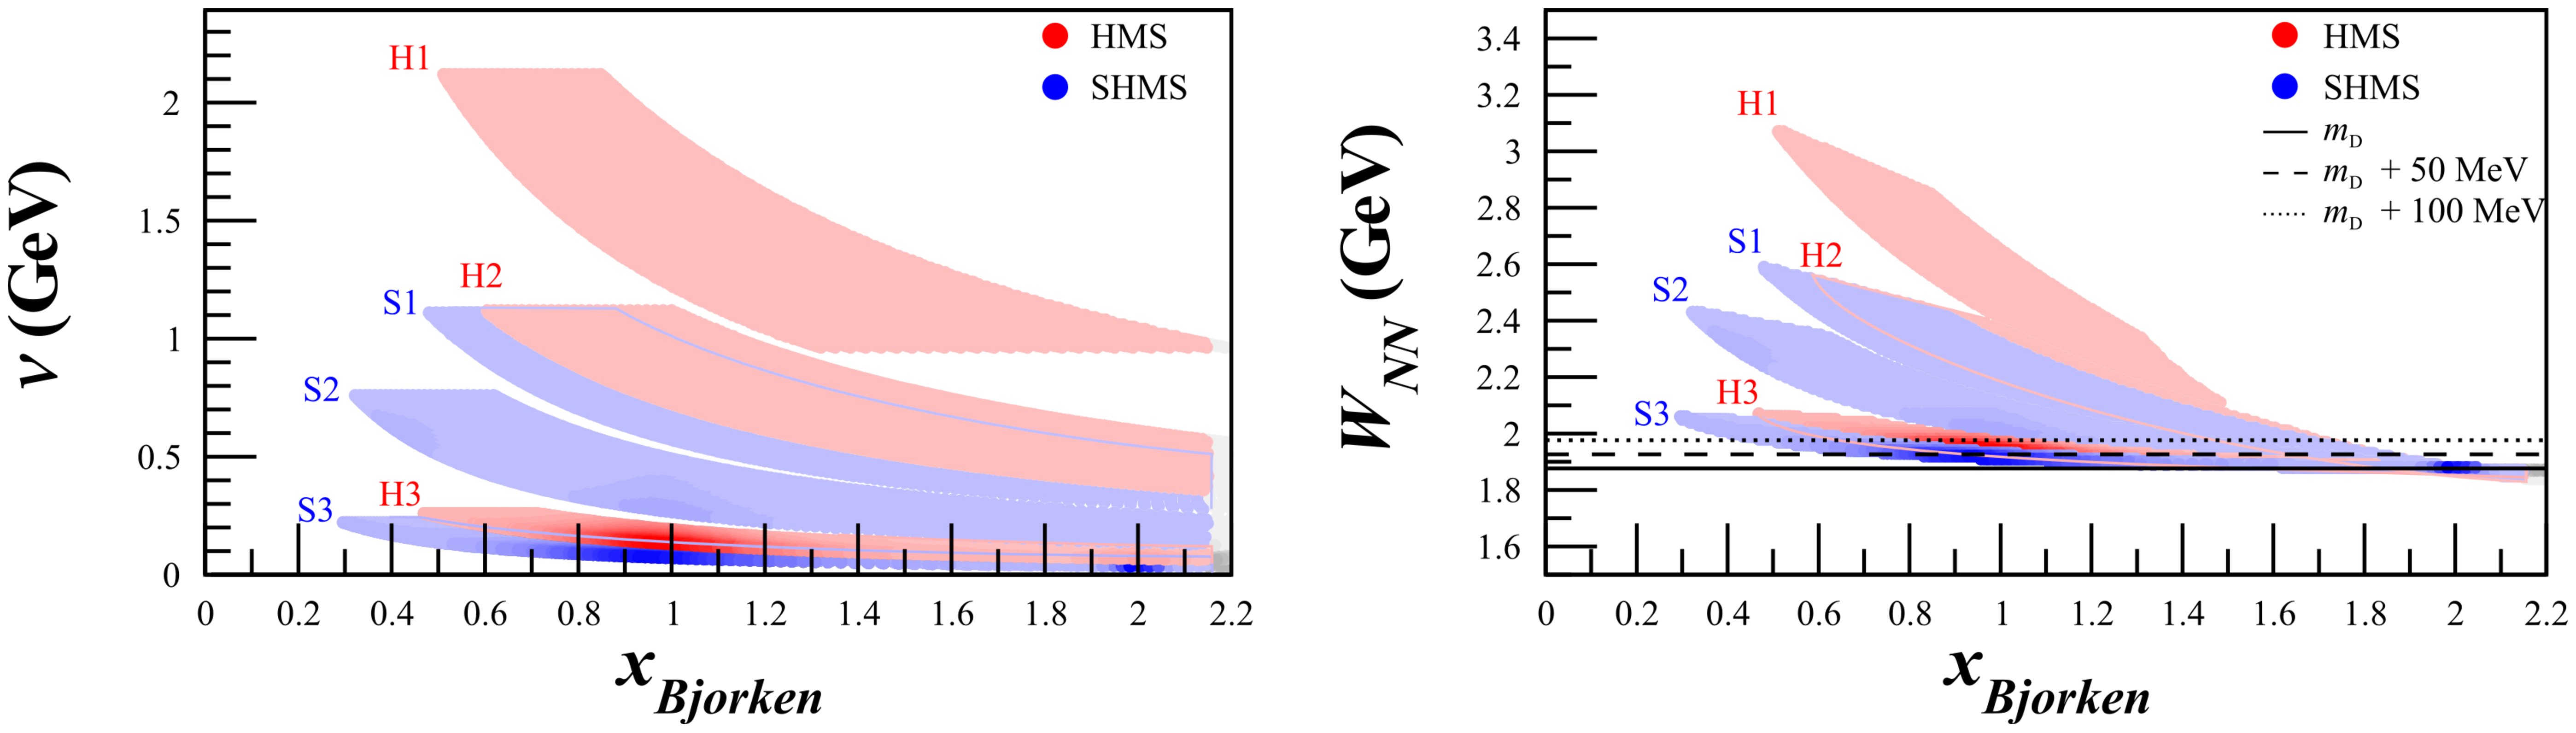
\includegraphics[width=\textwidth]{figs/Pzz_30_all_nu_wnn.eps}
%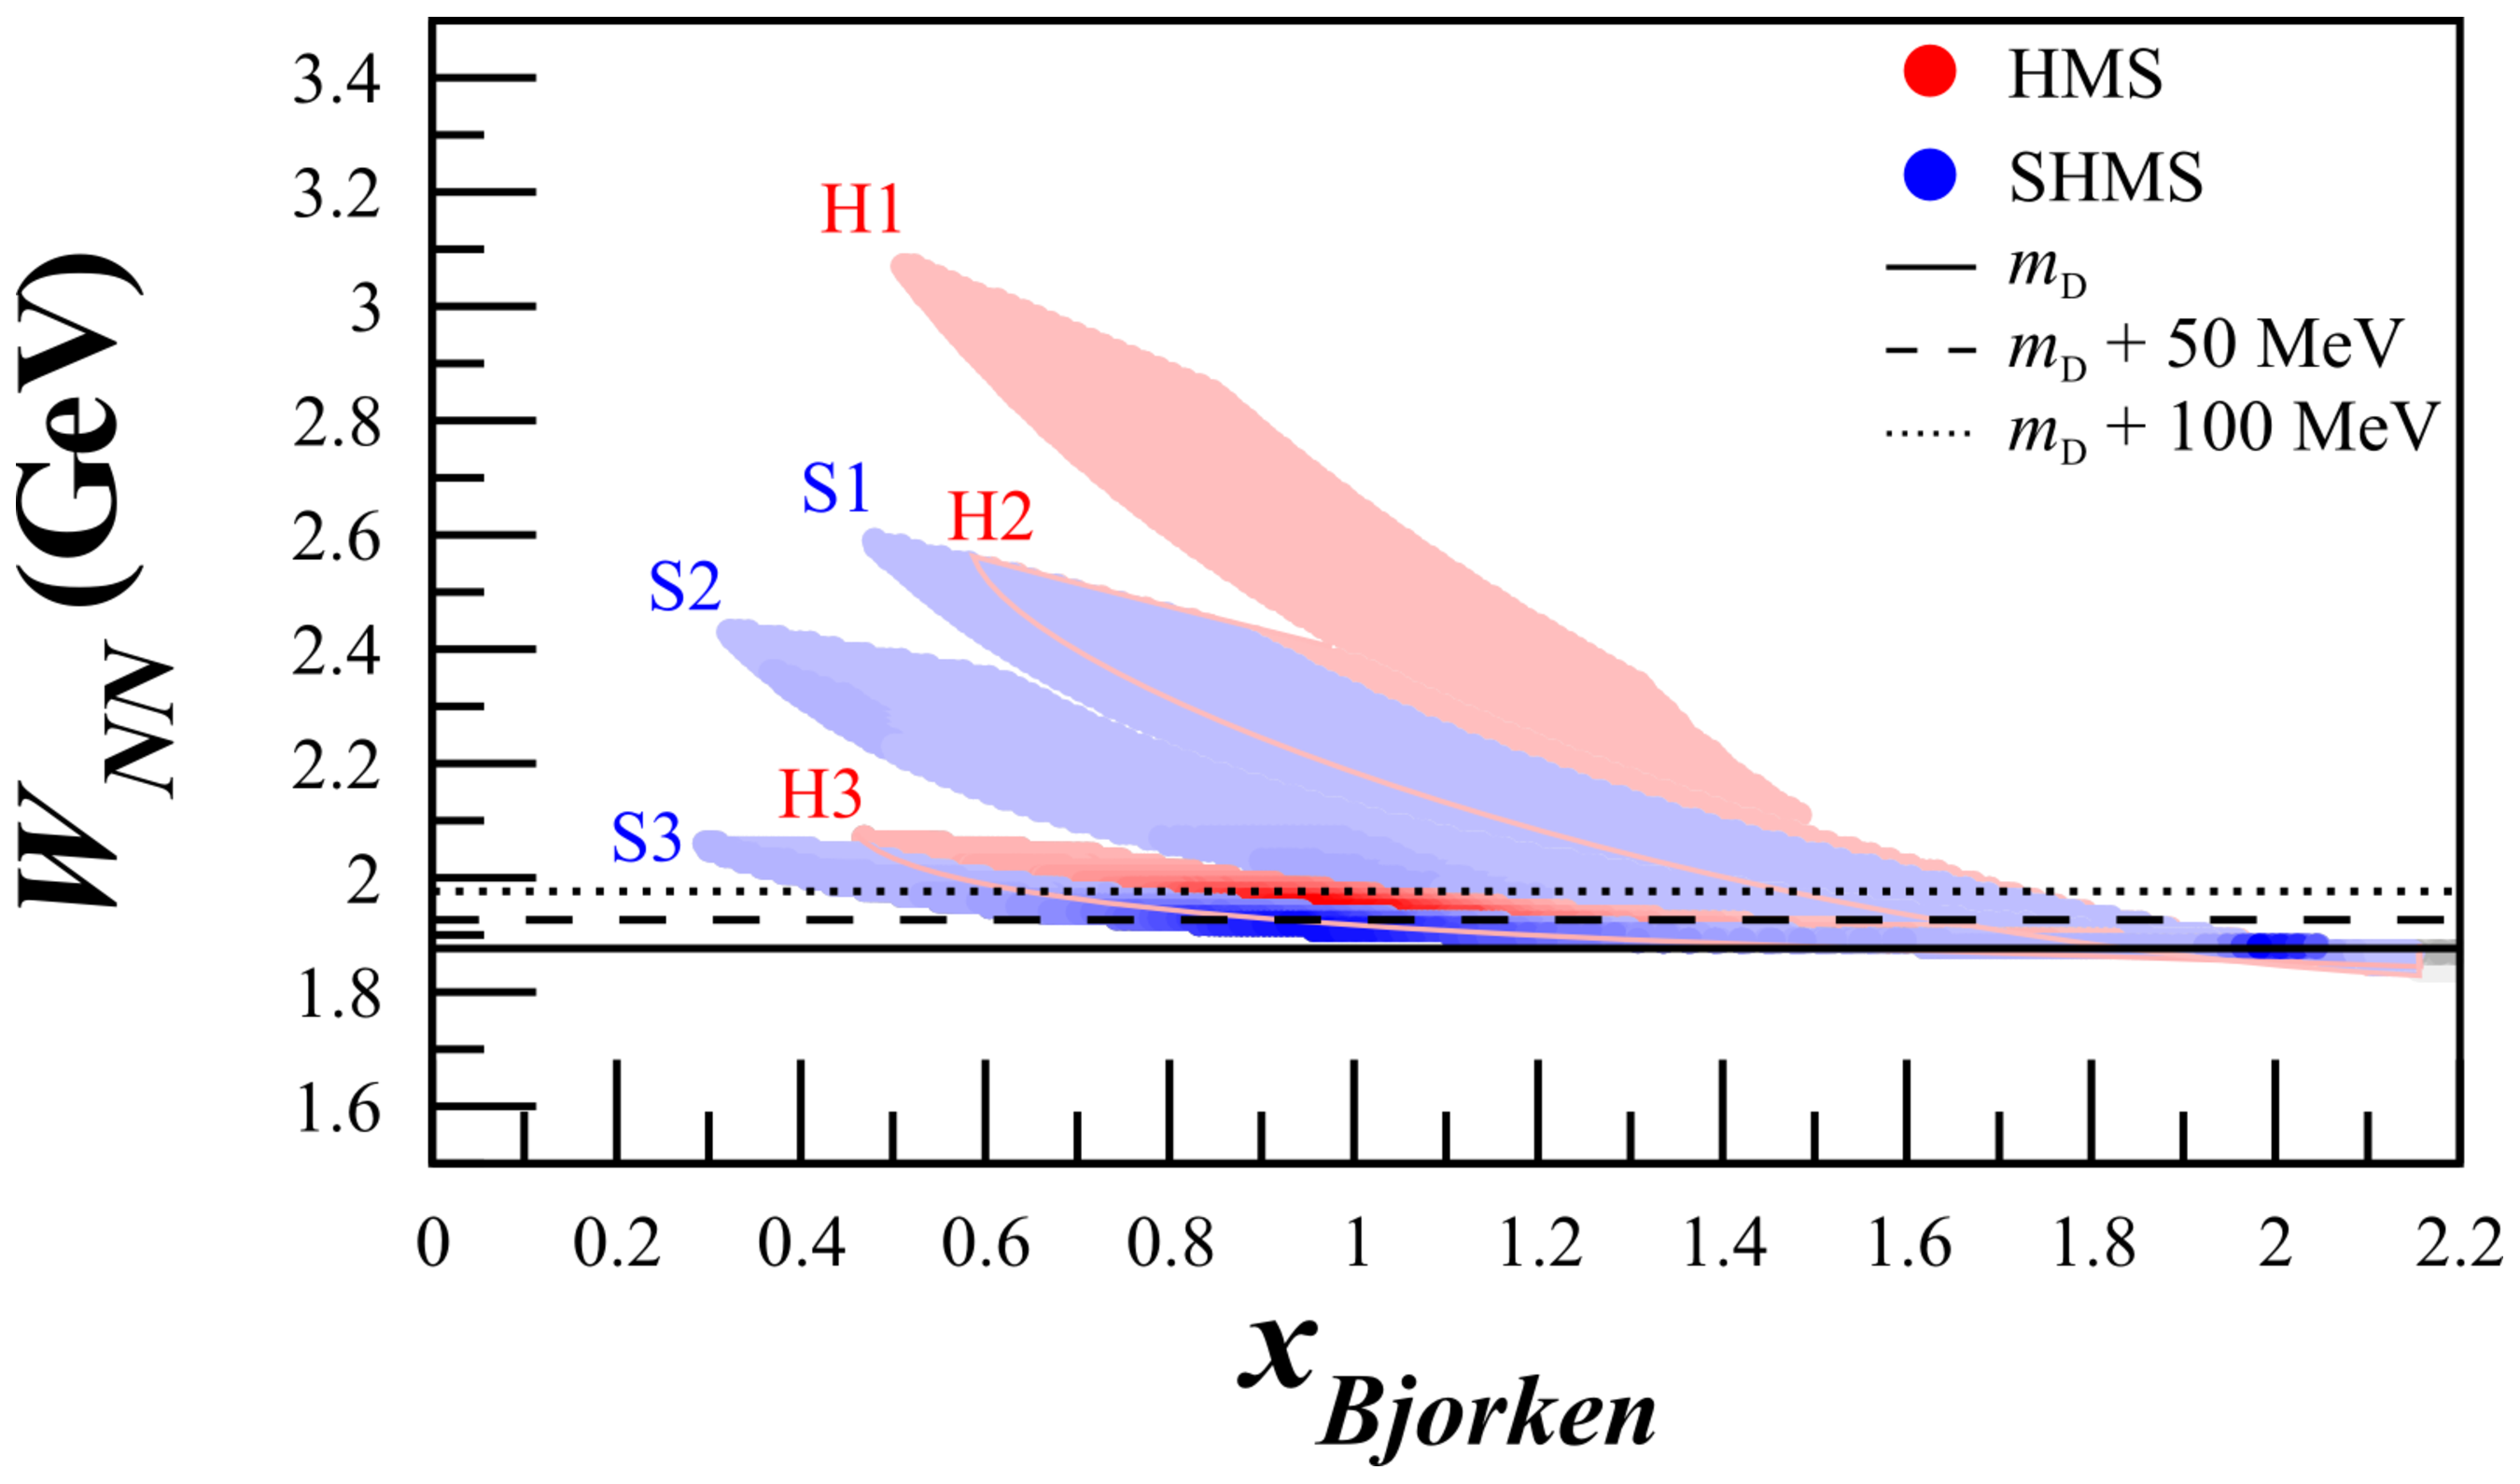
\includegraphics[width=0.49\textwidth]{figs/Pzz_30_all_wnn.eps} %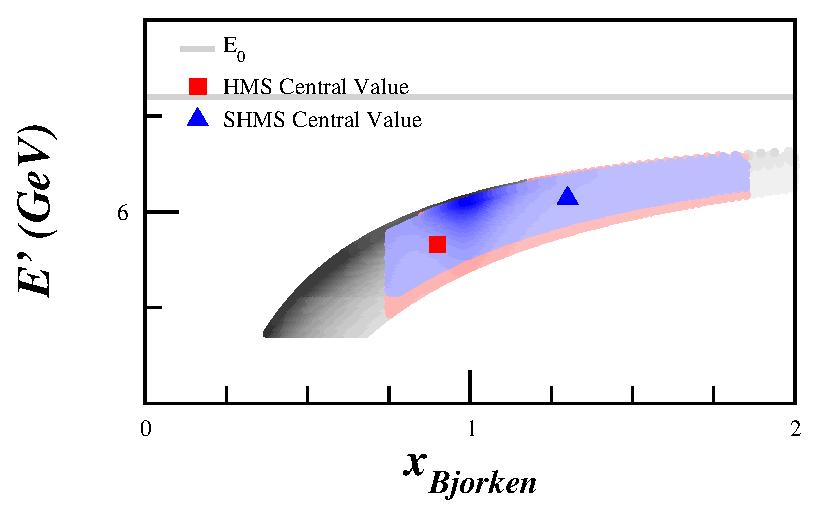
\includegraphics[width=0.49\textwidth]{figs/kine/Pzz_30_eprime.eps}
%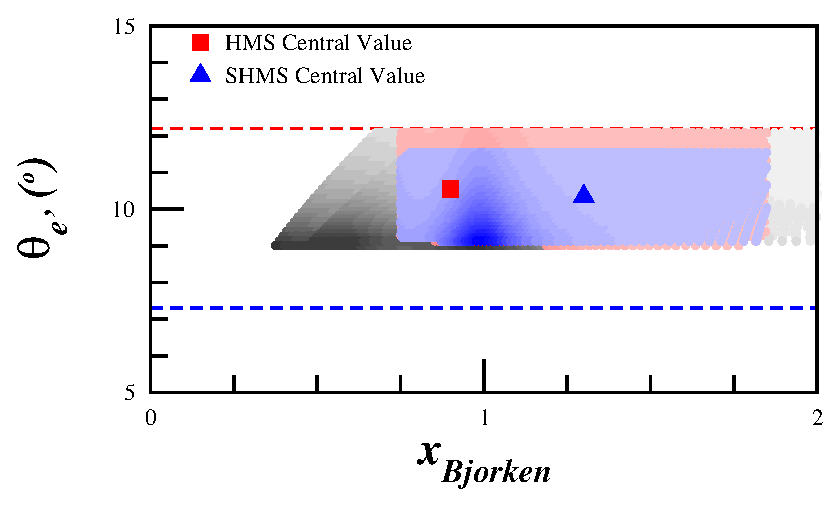
\includegraphics[width=0.49\textwidth]{figs/kine/Pzz_30_theta_eprime.eps}~~ 

\caption{\label{kincov} Kinematic coverage for central spectrometer settings at $Q^2=2.9~(\mathrm{GeV}/c)^2$ (H1), $1.8~(\mathrm{GeV}/c)^2$ (H2), $1.5~(\mathrm{GeV}/c)^2$ (S1), $0.7~(\mathrm{GeV}/c)^2$ (S2), $0.3~(\mathrm{GeV}/c)^2$ (H3), and $0.2~(\mathrm{GeV}/c)^2$ (S3). The grey regions are not included in our statistics estimates since they fall outside the range of electron-deuteron scattering. Darker shading represents areas with higher statistics. The solid, dashed, and dotted lines in the $W_{NN}$ plot indicate deuteron mass, deuteron mass + 50 MeV, and deuteron mass + 100 MeV, respectively. Virtual-nucleon and light cone calculations are only valid for $W_{NN}>m_D+50$~MeV.}
\end{center}
\end{figure}

Although it has been pointed out that the current construction of the SHMS constrains it to angles $>10\%$ due to fringe fields affecting the beam entering the dump~\cite{Moore:2014sxa}, this can be resolved in a number of ways. As discussed in \cite{Moore:2014sxa}, passive iron shielding can be installed within the SHMS that would not affect the target field. Additionally, given the low beam current proposed, a local beam dump could be installed immediately following the target. In the worst case, we could meet the physics motivation by keeping the same $Q^2$ ranges as S1, S2, and S3 but lowering the highest beam energies while putting the SHMS at larger angles. In this case, the HMS would be used at very similar angles to combine statistics between the spectrometers to make up for the loss in statistics from the SHMS. 


The polarized \TARGET target is discussed in Section~\ref{POLTARGSEC}.  The magnetic field of the target will be held constant along the beamline at all times, while the target state is alternated between a polarized and unpolarized state.
The tensor polarization and packing fraction used in the rates estimate are \PZZ\% and \PF, respectively. 
The dilution factor in the range of this measurement is shown in Fig.~\ref{fdil_plot}. The spread of the elastic peak for the dilution factor was calculated assuming a momentum resolution of $0.1\%$ for the HMS and $0.08\%$ for the SHMS.
With an incident electron beam current of \CURRENT nA, the expected deuteron luminosity is \LUMI.


%$1.57\times 10^{35}$~cm$^{-2}}$s$^{-1}$.
%$?.??\times 10^{35}$~cm$^{-2}$s$^{-1}$.

\begin{figure}
\begin{center}
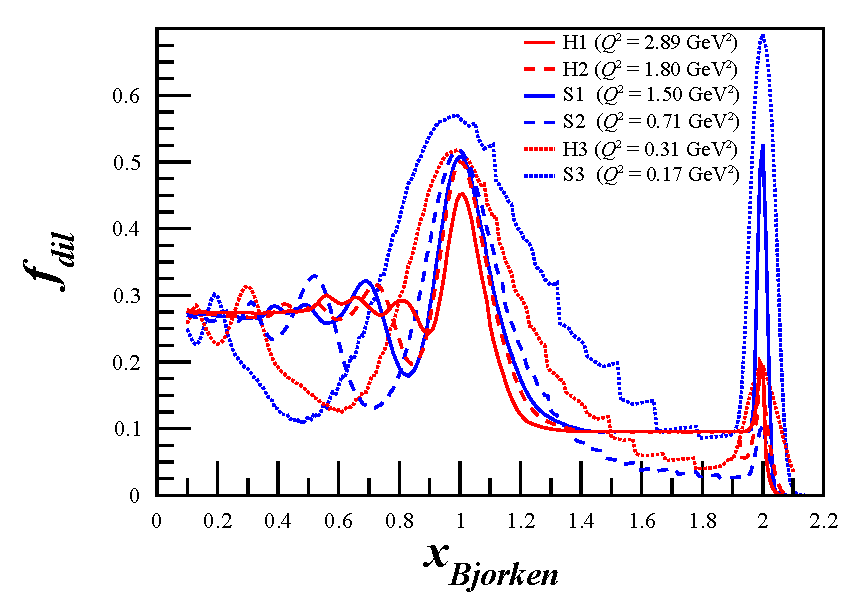
\includegraphics[width=0.65\textwidth]{figs/Pzz_30_fdil_all.eps} 
\caption{\label{fdil_plot}Projected dilution factor covering the entire $x$ range to be measured using a combination of P. Bosted's~\cite{Bosted:2012qc} and M. Sargsian's~\cite{misak-convo} code, along with a calculation of the elastic peak using a parametrization of the deuteron form factors, for the SHMS and HMS.}
\end{center}
\end{figure}


The momentum bite and the acceptance were assumed to be $\Delta P = \pm 8\%$ and $\Delta\Omega = 5.6$~msr for the HMS, and $\Delta P= ^{+20\%}_{-8\%}$ 
%$-8<\Delta P <+20\%$
and $\Delta\Omega =4.4$~msr for the SHMS. 
%
For the choice of the kinematics,
special attention was taken onto the angular and momentum limits of the spectrometers with a longitudinal polarized target: for the
HMS, $12.2^{\circ} \le \theta \le 85^{\circ}$ and $1 \le P_0 \le 7.3$ GeV/c, and for the SHMS,
$5.5^{\circ} \le \theta \le 40^{\circ}$ and $2 \le P_0 \le 11$ GeV/c. In addition, the
opening angle between the spectrometers is physically constrained to be larger than 17.5$^{\circ}$.

A total of \productiondays days of beam time is requested for production data, with an additional \overheaddays days of expected overhead. The expected uncertainties, described in detail in Section~\ref{uncertainties}, are given in Tables~\ref{RATES2}-\ref{RATES-T20} and Figs.~\ref{PROJ}-\ref{PROJ-T20}.

\begin{table}
\begin{center}
\begin{tabular}{c|ccc|ccc|ccc}
 ~ & \multicolumn{3}{|c}{H1: $Q^2=2.9\mathrm{~(GeV/}c)^2$} & \multicolumn{3}{|c}{H2: $Q^2=1.8\mathrm{~(GeV/}c)^2$} & \multicolumn{3}{|c}{S1: $Q^2=1.5\mathrm{~(GeV/}c)^2$} \\
 \hline
  $x$  & $f_{dil}$ & $\delta A_{zz}^{stat}$ & $\delta A_{zz}^{sys}$ & $f_{dil}$ & $\delta A_{zz}^{stat}$ & $\delta A_{zz}^{sys}$ & $f_{dil}$ & $\delta A_{zz}^{stat}$ & $\delta A_{zz}^{sys}$ \\
  &     & $\times 10^{-2}$  & $\times 10^{-2}$  &    & $\times 10^{-2}$  & $\times 10^{-2}$ &    & $\times 10^{-2}$  & $\times 10^{-2}$ \\
\hline\hline
%       |         Q2=2.9         |      Q2=1.8           |      Q2=1.5
%  x  	   fdil 	   dAzz	 dAzzSys  fdil 	  dAzz   dAzzSys  fdil   dAzz	 dAzzSys
 0.50   &  0.29	 & 2.02	& 1.84	& ---	& ---	& ---	& 0.25	& 0.72	& 1.84 \\
 0.60   &  0.29	 & 0.91	& 0.10	& 0.27	& 3.15	& 0.10	& 0.30	& 0.36	& 0.10 \\ 
 0.70   &  0.27	 & 1.01	& 0.10	& 0.32	& 1.26	& 0.10	& 0.29	& 0.38	& 0.10 \\
 0.80	&  0.30	 & 1.11	& 1.34	& 0.20	& 2.00	& 0.48	& 0.17	& 0.74	& 1.34 \\
 0.90	&  0.24	 & 1.73 	& 0.38 	& 0.27	& 1.45	& 1.10	& 0.29	& 0.44	& 0.38 \\
 1.00	&  0.46	 & 1.03	& 0.10 	& 0.50	& 0.74	& 0.10	& 0.51	& 0.24	& 0.10 \\
 1.10	&  0.28	 & 2.48	& 0.14 	& 0.33	& 1.58	& 1.65	& 0.34	& 0.49	& 0.14 \\
 1.20	&  0.09	 & 11.7	& 1.55 	& 0.10	& 7.18	& 3.31	& 0.17	& 1.34	& 1.55 \\
 1.30	&  0.11	 & 16.8	& 4.13 	& 0.11	& 9.76	& 4.96	& 0.12	& 2.79	& 4.13 \\
 1.40	&  ---	 & ---	& --- 	& 0.12	& 15.1	& 6.65	& 0.13	& 4.30	& 6.72 \\
 1.50	&  ---	 & ---	& ---	& 0.11	& 19.8	& 8.29	& 0.10	& 7.01	& 8.34 \\
 1.60	&  ---	 & ---	& --- 	& ---	& ---	& ---	& 0.10	& 9.60	& 8.42 \\
 1.70	&  ---	 & ---	& --- 	& ---	& ---	& ---	& 0.10	& 12.7	& 7.04 \\
 1.80	&  ---	 & ---	& --- 	& ---	& ---	& ---	& 0.10	& 16.6	& 4.72 \\
 2.00   &  ---	 & ---	& ---	& 0.20	& 9.33	& 9.20	& 0.50	& 2.79	& 9.20 \\
\hline\hline
\end{tabular}
\caption{\label{RATES2}Summary of the expected uncertainty for each $x$ bin for settings S1, H1, and H2. }
\end{center}
\end{table}

\begin{table}
\begin{center}
\begin{tabular}{c|ccc|ccc|ccc}
 ~ & \multicolumn{3}{|c}{S2: $Q^2=0.7\mathrm{~(GeV/}c)^2$} & \multicolumn{3}{|c}{H3: $Q^2=0.3\mathrm{~(GeV/}c)^2$} & \multicolumn{3}{|c}{S3: $Q^2=0.2\mathrm{~(GeV/}c)^2$} \\
 \hline
  $x$  & $f_{dil}$ & $\delta A_{zz}^{stat}$ & $\delta A_{zz}^{sys}$ & $f_{dil}$ & $\delta A_{zz}^{stat}$ & $\delta A_{zz}^{sys}$ & $f_{dil}$ & $\delta A_{zz}^{stat}$ & $\delta A_{zz}^{sys}$ \\
  &     & $\times 10^{-2}$  & $\times 10^{-2}$  &    & $\times 10^{-2}$  & $\times 10^{-2}$ &    & $\times 10^{-2}$  & $\times 10^{-2}$ \\
\hline\hline
%       |         Q2=0.7         |      Q2=0.3           |      Q2=0.2
%  x  	   fdil 	   dAzz	 dAzzSys  fdil 	  dAzz   dAzzSys  fdil   dAzz	 dAzzSys
 0.30   &  0.24	 & 0.99	& 1.84	& ---	& ---	& ---	& 0.18	& 2.13	& 1.84 \\
 0.40   &  0.28	 & 0.26	& 1.84	& ---	& ---	& ---	& 0.12	& 1.38	& 1.84 \\
 0.50   &  0.32	 & 0.21	& 1.84	& 0.14	& 3.52	& 1.84	& 0.11	& 1.23	& 1.84 \\
 0.60   &  0.19	 & 0.41	& 0.10	& 0.12	& 2.26	& 0.10	& 0.18	& 0.78	& 0.10 \\ 
 0.70   &  0.13	 & 0.68	& 0.10	& 0.18	& 1.33	& 0.10	& 0.28	& 0.48	& 0.10 \\
 0.80	&  0.19	 & 0.48	& 0.48	& 0.30	& 0.72	& 0.48	& 0.42	& 0.31	& 0.48 \\
 0.90	&  0.39	 & 0.22 	& 1.10 	& 0.46	& 0.45	& 1.10	& 0.54	& 0.24	& 1.10 \\
 1.00	&  0.52	 & 0.16	& 0.10 	& 0.52	& 0.43	& 0.10	& 0.58	& 0.25	& 0.10 \\
 1.10	&  0.39	 & 0.28	& 1.27 	& 0.43	& 0.63	& 1.07	& 0.53	& 0.33	& 0.95 \\
 1.20	&  0.22	 & 0.65	& 2.54 	& 0.30	& 1.15	& 2.14	& 0.40	& 0.55	& 1.91 \\
 1.30	&  0.14	 & 1.34	& 3.81 	& 0.19	& 2.16	& 3.22	& 0.32	& 0.83	& 2.87 \\
 1.40	&  0.09	 & 2.29	& 5.06 	& 0.14	& 3.52	& 4.29	& 0.24	& 1.31	& 3.82 \\
 1.50	&  0.06	 & 4.09	& 6.35	& 0.10	& 5.85	& 5.37	& 0.20	& 1.86	& 4.78 \\
 1.60	&  0.04	 & 7.76	& 7.60 	& 0.06	& 10.4	& 6.45	& 0.14	& 2.87	& 5.74 \\
 1.70	&  0.04	 & 9.23	& 8.88 	& 0.05	& 13.5	& 7.52	& 0.10	& 4.53	& 6.69 \\
 1.80	&  0.03	 & 14.9	& 9.20 	& 0.06	& 13.9	& 8.60	& 0.11	& 4.73	& 7.66 \\
 2.00   &  0.67	 & 3.79	& 9.20	& 0.20	& 3.05	& 9.20	& 0.70	& 0.45	& 9.20 \\
\hline\hline
\end{tabular}
\caption{\label{RATES3}Summary of the expected uncertainty for each $x$ bin for settings S2, S3, and H3. }
\end{center}
\end{table}


\begin{figure}
\begin{center}
%\includegraphics[width=0.45\textwidth]{figs/plots0705/b1_proj_newmiller_lin.eps}
%\hspace{0.5cm}
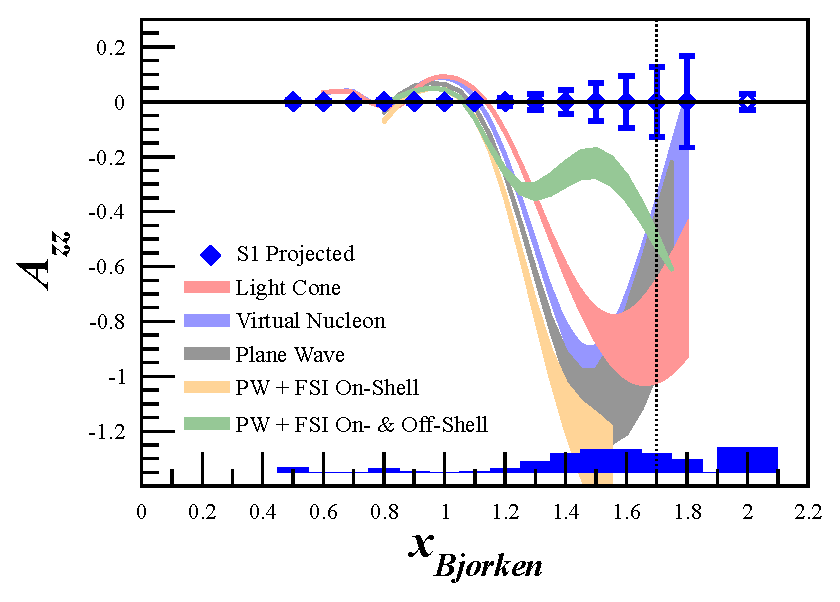
\includegraphics[width=0.49\textwidth]{figs/Azz_S1.eps}
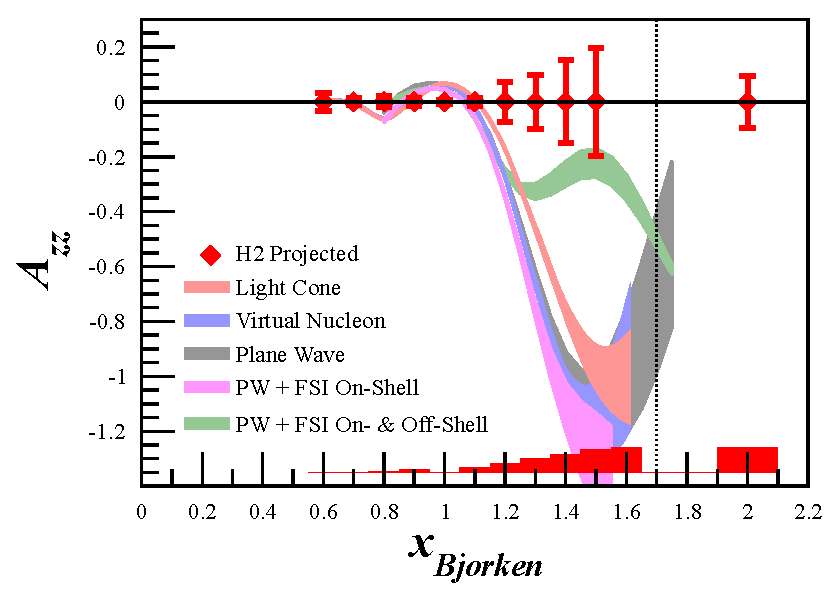
\includegraphics[width=0.49\textwidth]{figs/Azz_H2.eps}
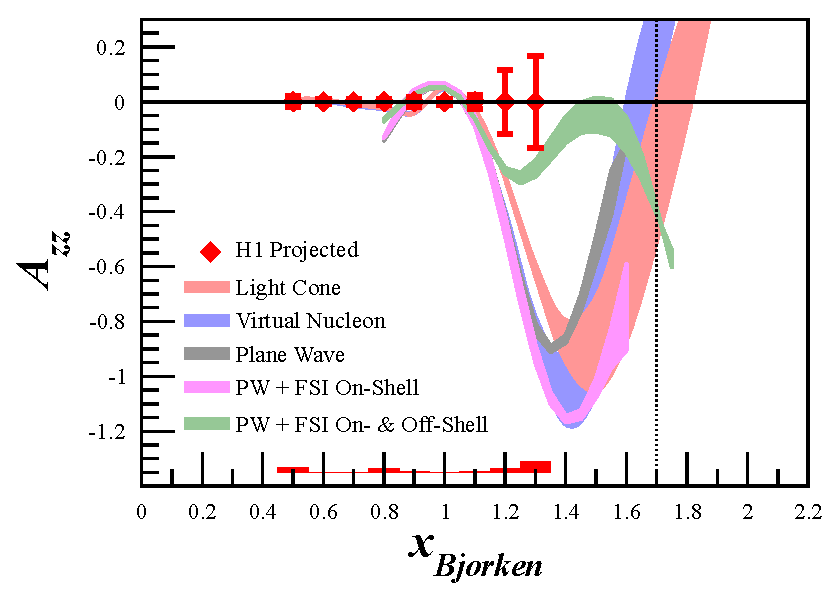
\includegraphics[width=0.49\textwidth]{figs/Azz_H1.eps}
 %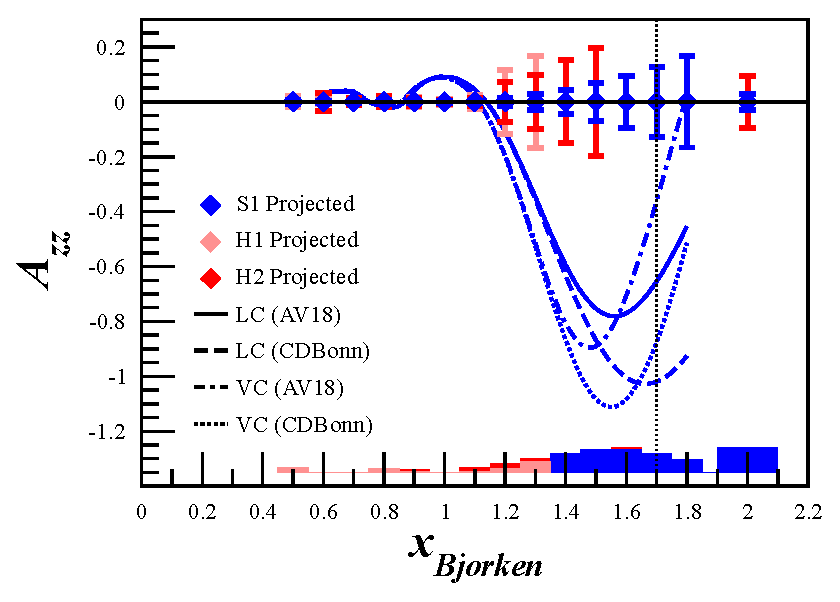
\includegraphics[width=0.49\textwidth]{figs/Azz_S1_H1_H2_vn_lc.eps} 
%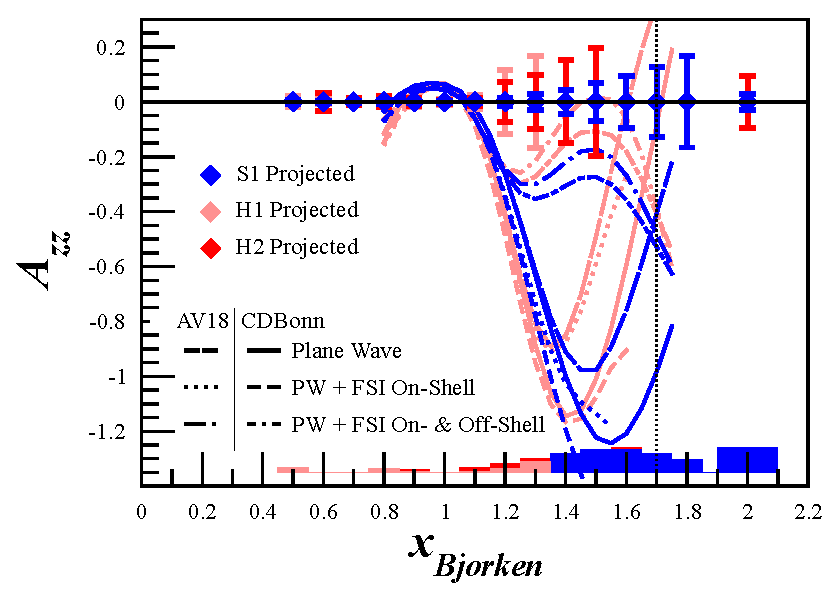
\includegraphics[width=0.49\textwidth]{figs/Azz_S1_H1_H2_fsi.eps} \\
\includegraphics[width=0.49\textwidth]{figs/Azz_S2_H3_S3.eps} 
\caption{\label{PROJ}Projected uncertainties for the tensor asymmetry $A_{zz}$ with \productiondays days of beam time for SHMS settings S1, S2, and S3, and HMS settings H1, H2, and H2 as described in Table~\ref{RATES1}. The bottom band represents the systematic uncertainty. The bands for the theoretical calculations show the spread based on the choice of NN potentials. The upper $x$ limit for H1 (H2) is $x=1.3$ ($x=1.5$). Light-cone (LC) and virtual-nucleon (VN) calculations using the AV18 and CDBonn potentials were provided by M. Sargsian~\cite{Sargsian:2014fla}. The dotted line at $x=1.75$ indicates the threshold of $W_{NN}>m_D+50$~MeV where LC and VN calculations begin to not be valid as $A_{zz}$ approaches the elastic peak~\cite{Frankfurt:1993sp}. Final state interactions on the virtual-nucleon model were provided by W. Cosyn~\cite{cosyn-convo}, indicating the effects from on- and off-shell. The bottom-right plot includes a modified Frankfurt and Strikman model~\cite{Frankfurt:1988nt} that estimates the peak shifts in $x$ expected due to the SRC scaling changing with $Q^2$~\cite{Frankfurt:2008zv}.
}
\end{center}
\end{figure}

\begin{figure}
\begin{center}
%\includegraphics[width=0.45\textwidth]{figs/plots0705/b1_proj_newmiller_lin.eps}
%\hspace{0.5cm}
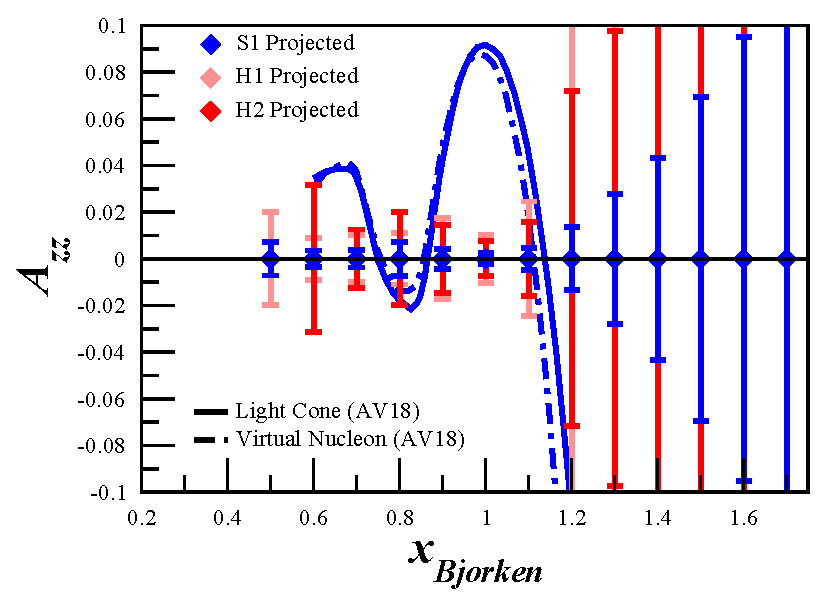
\includegraphics[width=0.49\textwidth]{figs/Azz_S1_H1_H2_zoom.eps} 
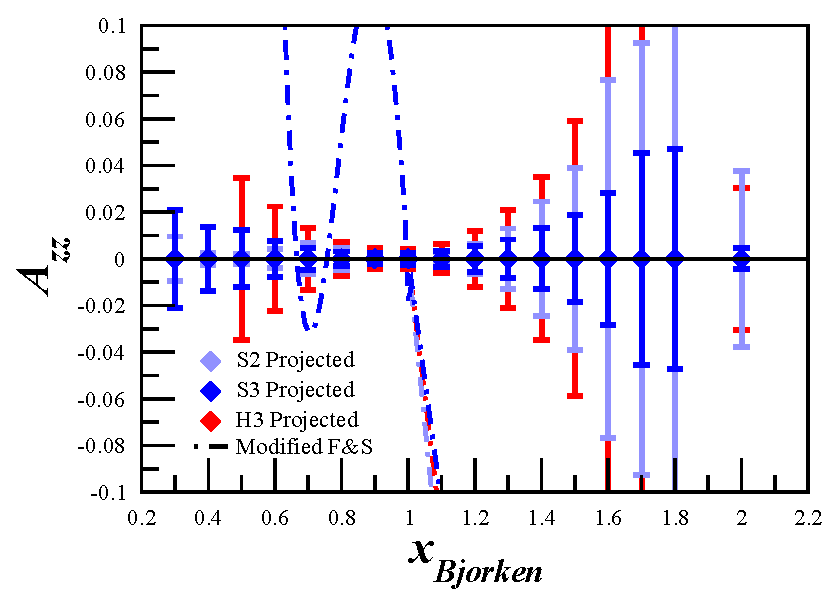
\includegraphics[width=0.49\textwidth]{figs/Azz_S2_H3_S3_zoom.eps} 
\caption{\label{PROJ-zoom}Projected uncertainties for the tensor asymmetry $A_{zz}$ with \productiondays days of beam time, same as in Figure~\ref{PROJ}, but zoomed in to $-0.1<A_{zz}<0.1$ to more clearly show the small uncertainties around the quasi-elastic peak.
}
\end{center}
\end{figure}

\begin{table}
\begin{center}
\begin{tabular}{c|c|c|c}
		& $Q^2$    	& $\delta T_{20}^{stat}$	&  $\delta T_{20}^{sys}$ \\
Setting	& (GeV$^2$)	& $\times 10^{-2}$		& $\times 10^{-2}$ \\
\hline\hline
H2 		& 1.8		&  21.7					& 4.74 \\  
S1 		& 1.5		&  6.09					& 4.77 \\
S2 		& 0.7		&  8.28					& 6.88 \\  
H3 		& 0.3		&  6.66					& 9.91 \\  
S3 		& 0.2		&  0.99					& 5.59 \\
  
\hline\hline
\end{tabular}
\caption{\label{RATES-T20}Expected uncertainties for $T_{20}$ assuming a systematic uncertainty of 9.2\%, which could be reduced further by utilizing the S3 measurement as a calibration for the polarized target.}
\end{center}
\end{table}

\begin{figure}
\begin{center}
%\includegraphics[width=0.45\textwidth]{figs/plots0705/b1_proj_newmiller_lin.eps}
%\hspace{0.5cm}
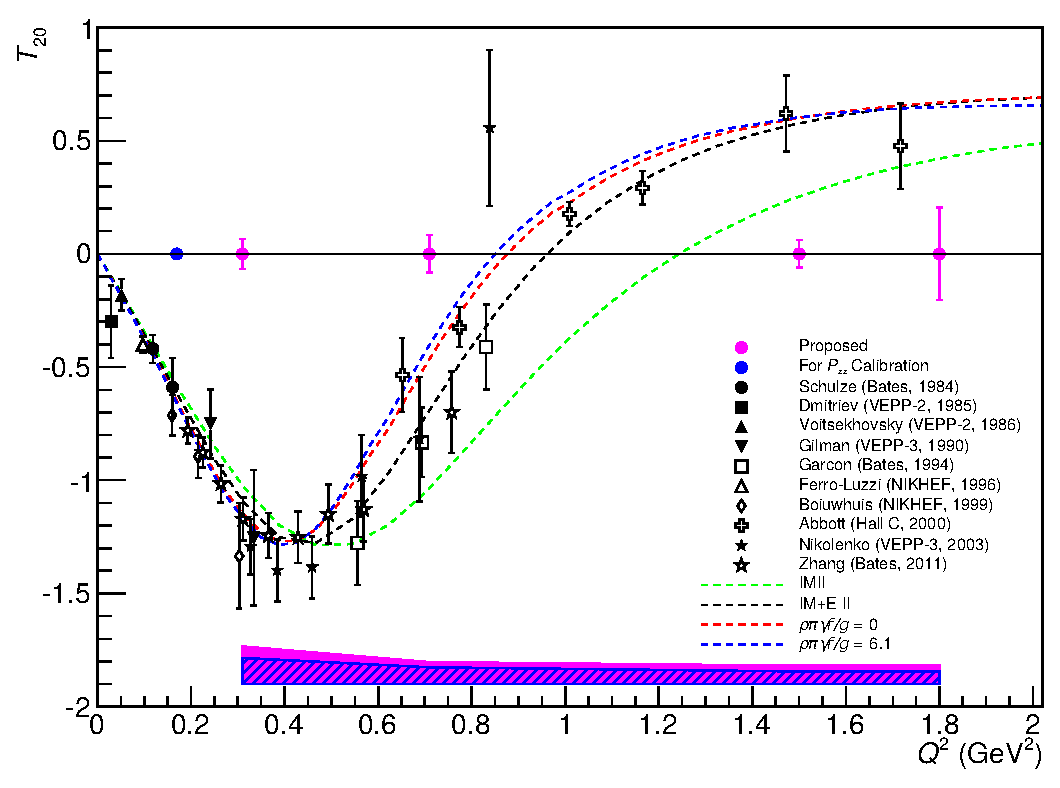
\includegraphics[width=\textwidth]{figs/plot_t20_fit.eps} 
\caption{\label{PROJ-T20}Projected uncertainties for the elastic tensor analyzing power $T_{20}$ with \productiondays days of beam time are shown alongside the world data~\cite{Holt:2012gg}. The point shown in blue, measured at $Q^2=0.2$~GeV$^2$ where $T_{20}$ is well known theoretically and experimentally, will be used as a calibration for $P_{zz}$, and can potentially be used to further reduce the leading systematic uncertainty as indicated by the blue-dashed band.
}
\end{center}
\end{figure}

\iffalse
\subsubsection{SHMS Angular Constraints}

It was recently pointed out that the SHMS is being built such that it would not be able to go to low angles without the magnets interfering with the beam dump~\cite{Moore:2014sxa}. In particular, angles below $\approx10^{\circ}$ would cause the beam to miss the dump. Although solutions have been proposed, including a passive system of adding extra iron to the magnet yokes and beam pipe to reduce field leakage, they have not yet been implemented. In the case that they are not installed by the time of running, we can utilize a slightly different set of kinematics that will cover most of the same $Q^2$ range as in Section~\ref{kinematics} but at lower beam energies and larger angles. Although less ideal, the physics motivation is still valid at the reduced kinematics and the rates still make for a compelling measurement, as shown in Table~\ref{RATES1-const} and Figs.~\ref{kincov-const}-\ref{PROJ-const}.

\begin{table}
\begin{center}
\begin{tabular}{cc|c|c|c|c|c|c}
 & & $E_0$ & $Q^2$    	& $E'$  &    $\theta_{e'}$  &  Rates   & PAC Time   \\
%& (GeV) & (GeV$^2$)  & (GeV)  &     (deg.)   &   (kHz)  & (hours) \\
& & (GeV) & (GeV$^2$)  & (GeV)  &     ($^{\circ}$)   &   (kHz)  & (Days) \\
%\multicolumn{2}{|c|}{$\times 10^{-2}$}
\hline\hline
% Spec  Set   E_0       Q^2      E'        Th         Rate      Time
SHMS & (S1') & 6.6	&  1.5	&  6.07	&    11.1  	&    0.13	&   25 \\
HMS  & (H1') & 6.6	&  1.8	&  5.96	&    12.3	&    0.09	&   25 \\  
%SHMS & (S2) & 4.4	&  0.6	&  4.20	&    10.1 	&    2.07	&   8 \\
SHMS & (S2') & 4.4	&  0.7	&  4.15	&    11.3 	&    0.90	&   8 \\
HMS  & (H2') & 4.4	&  0.8	&  4.11	&    12.2	&    0.80	&   8 \\
SHMS & (S3') & 2.2	&  0.2	&  2.15	&    10.9 	&    10.5	&   1 \\
HMS  & (H3') & 2.2	&  0.3	&  2.11	&    14.9	&    3.23	&   1 \\  
\hline\hline
\end{tabular}
\caption{\label{RATES1-const}Central kinematics if the SHMS is constrained to $>10^{\circ}$. The lowest settings (S3 and H3) are unchanged from Fig.~\ref{RATES1}.}
\end{center}
\end{table}

%


\begin{figure}
\begin{center}
%\includegraphics[width=\textwidth]{figs/Pzz_30_all_q2_w.eps}
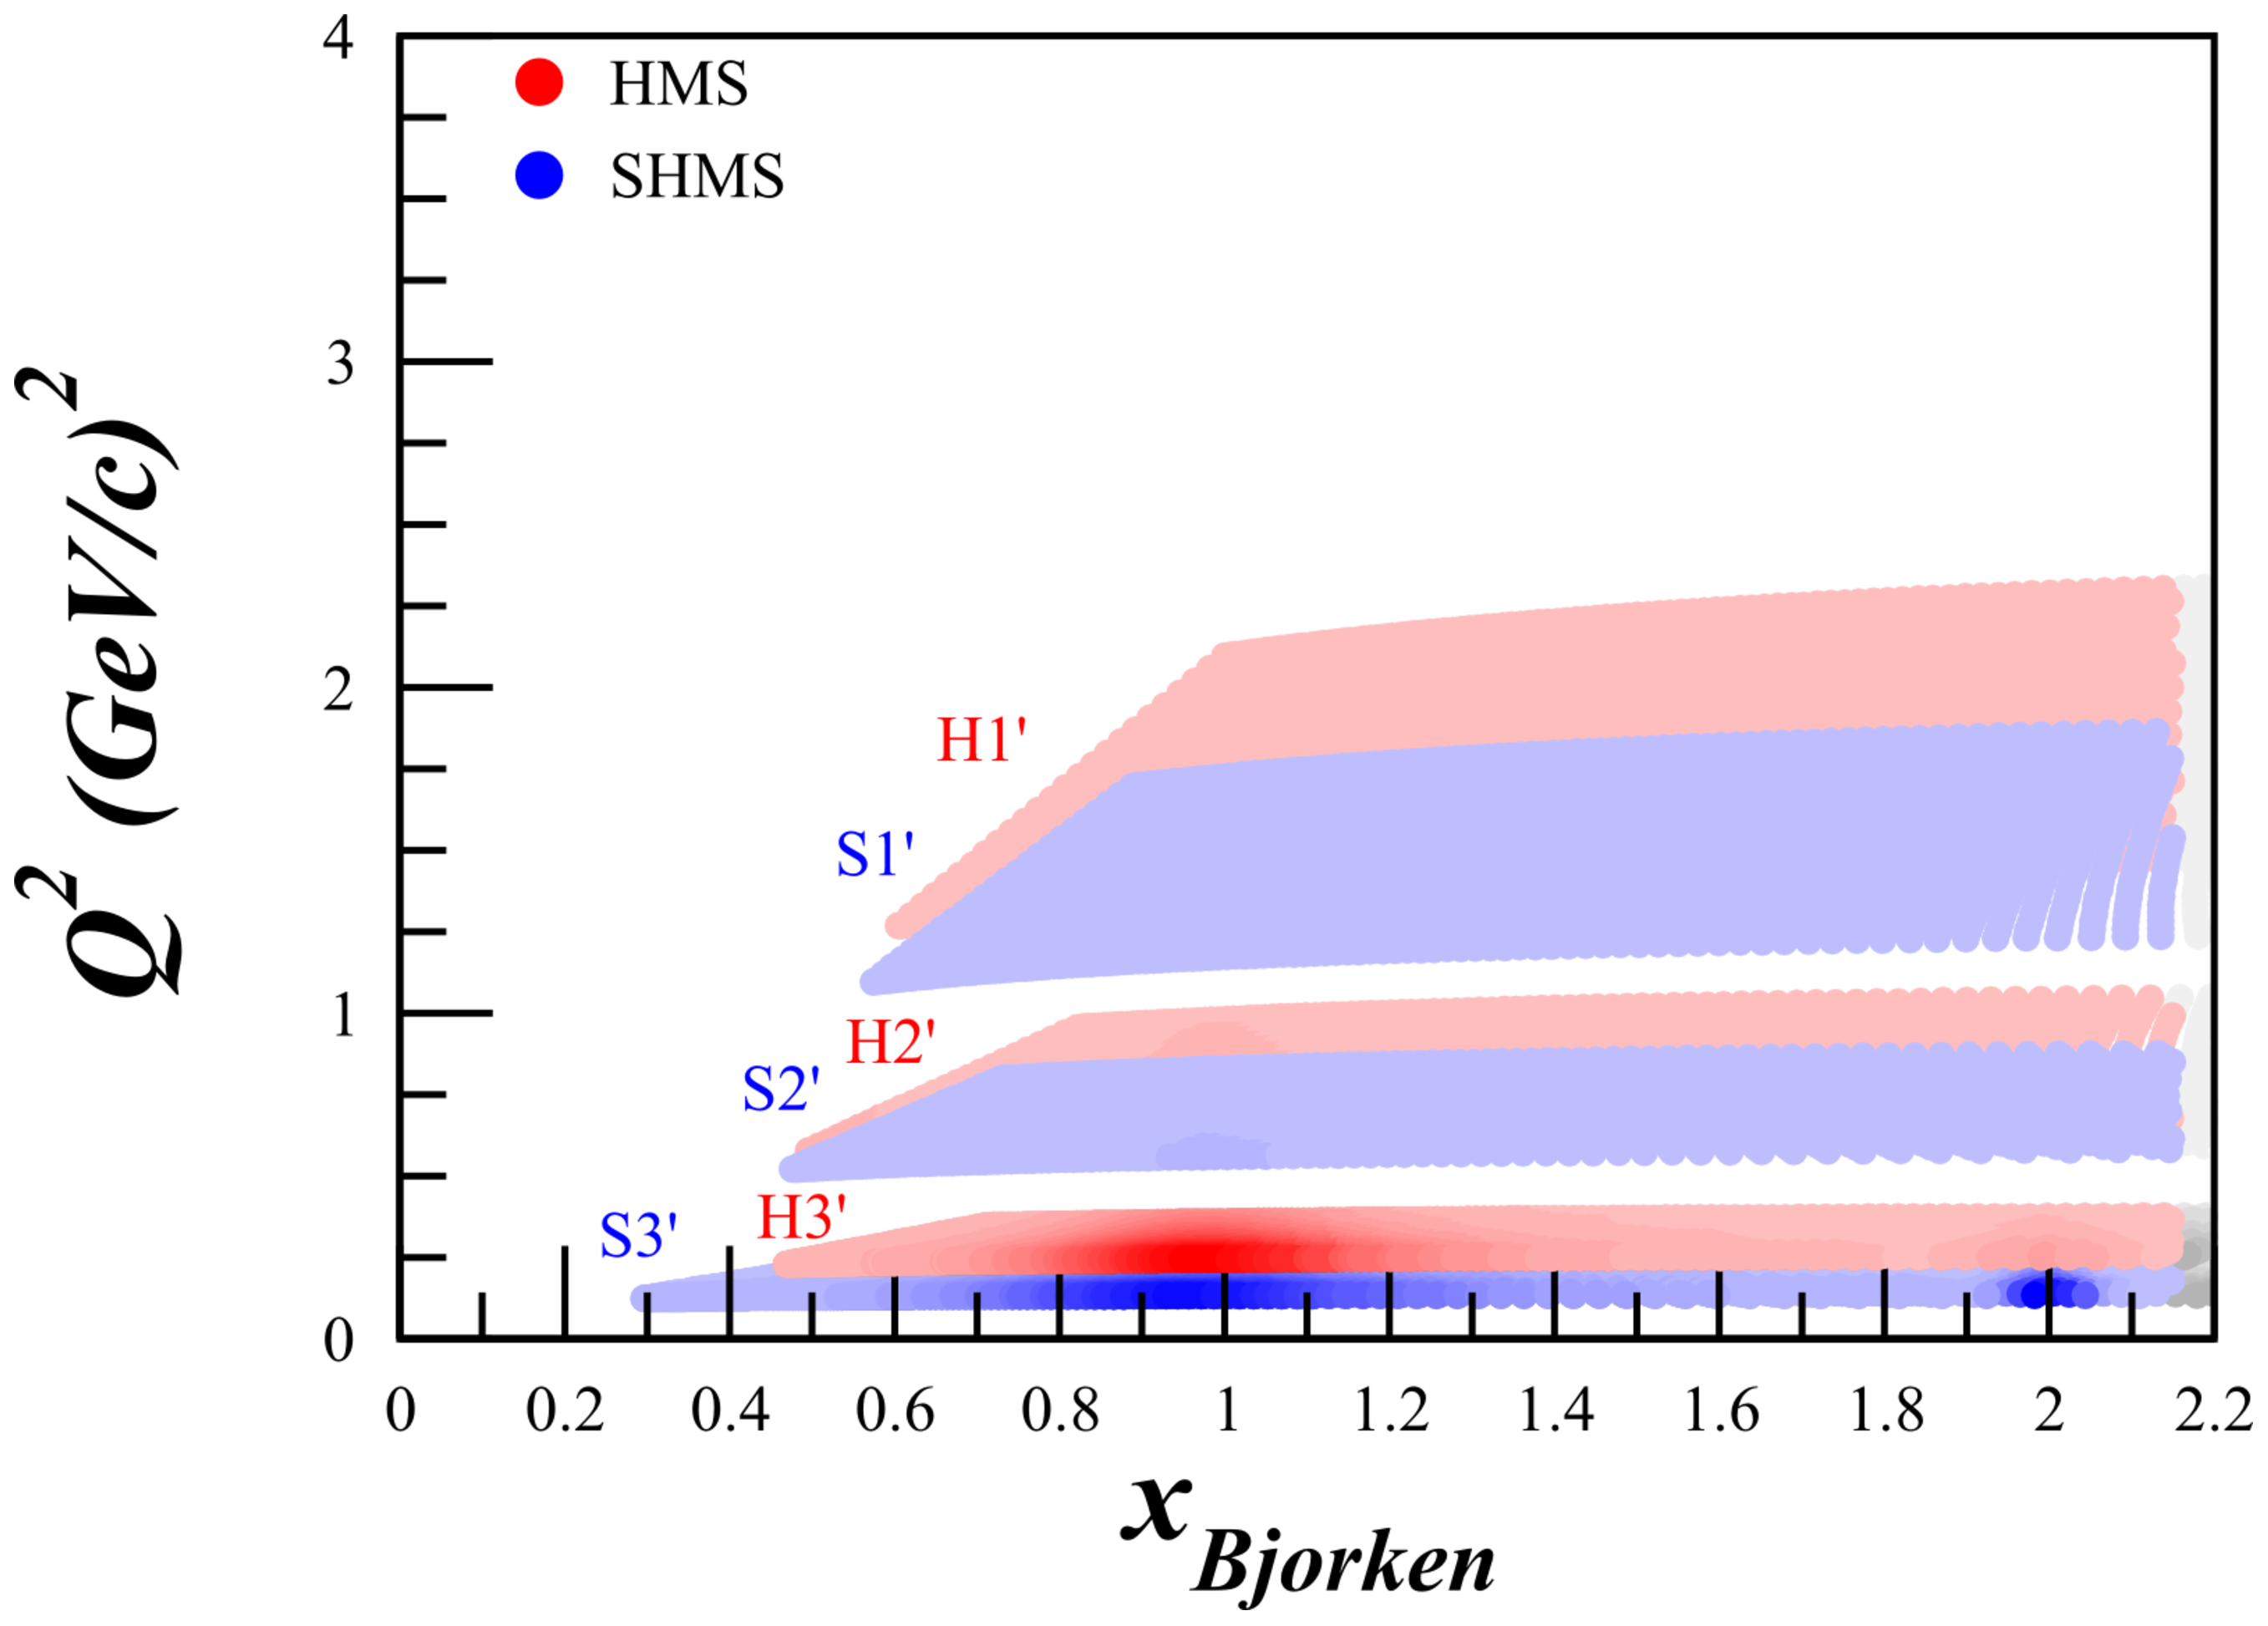
\includegraphics[width=0.49\textwidth]{figs/q2_shms_const.eps}

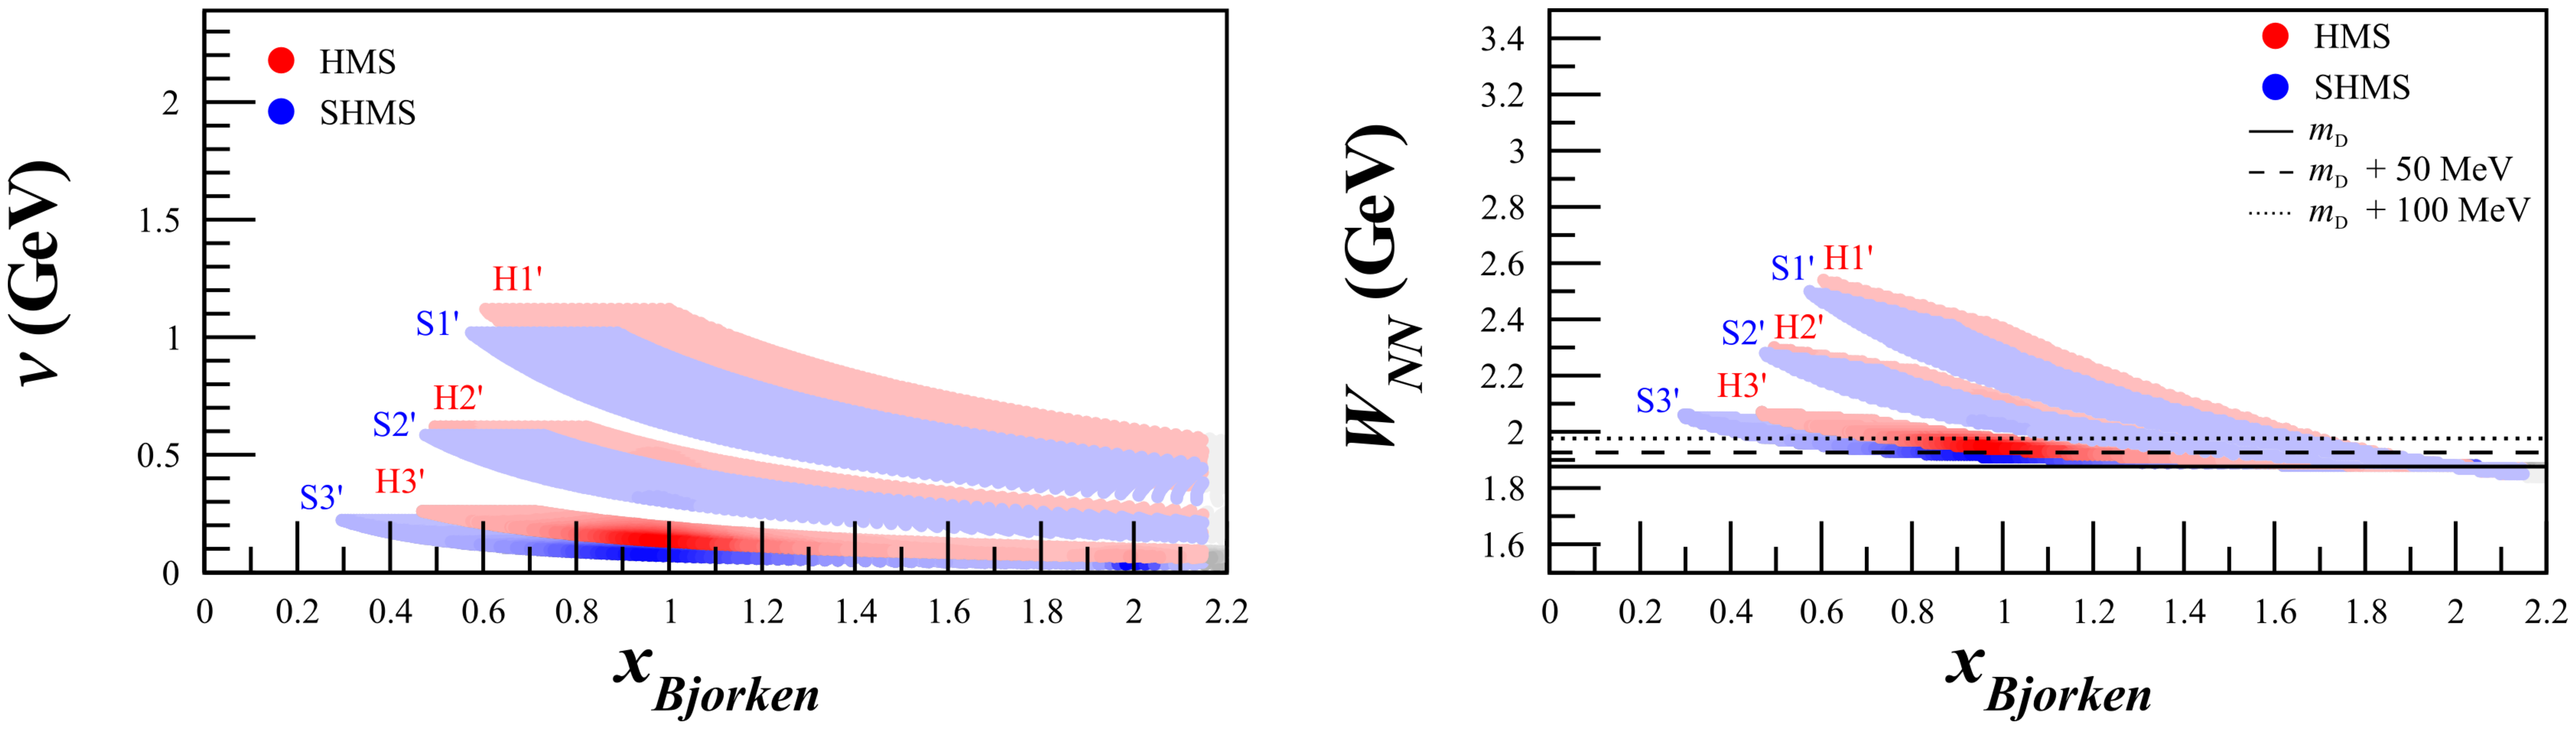
\includegraphics[width=\textwidth]{figs/nu_wnn_shms_const.eps}
%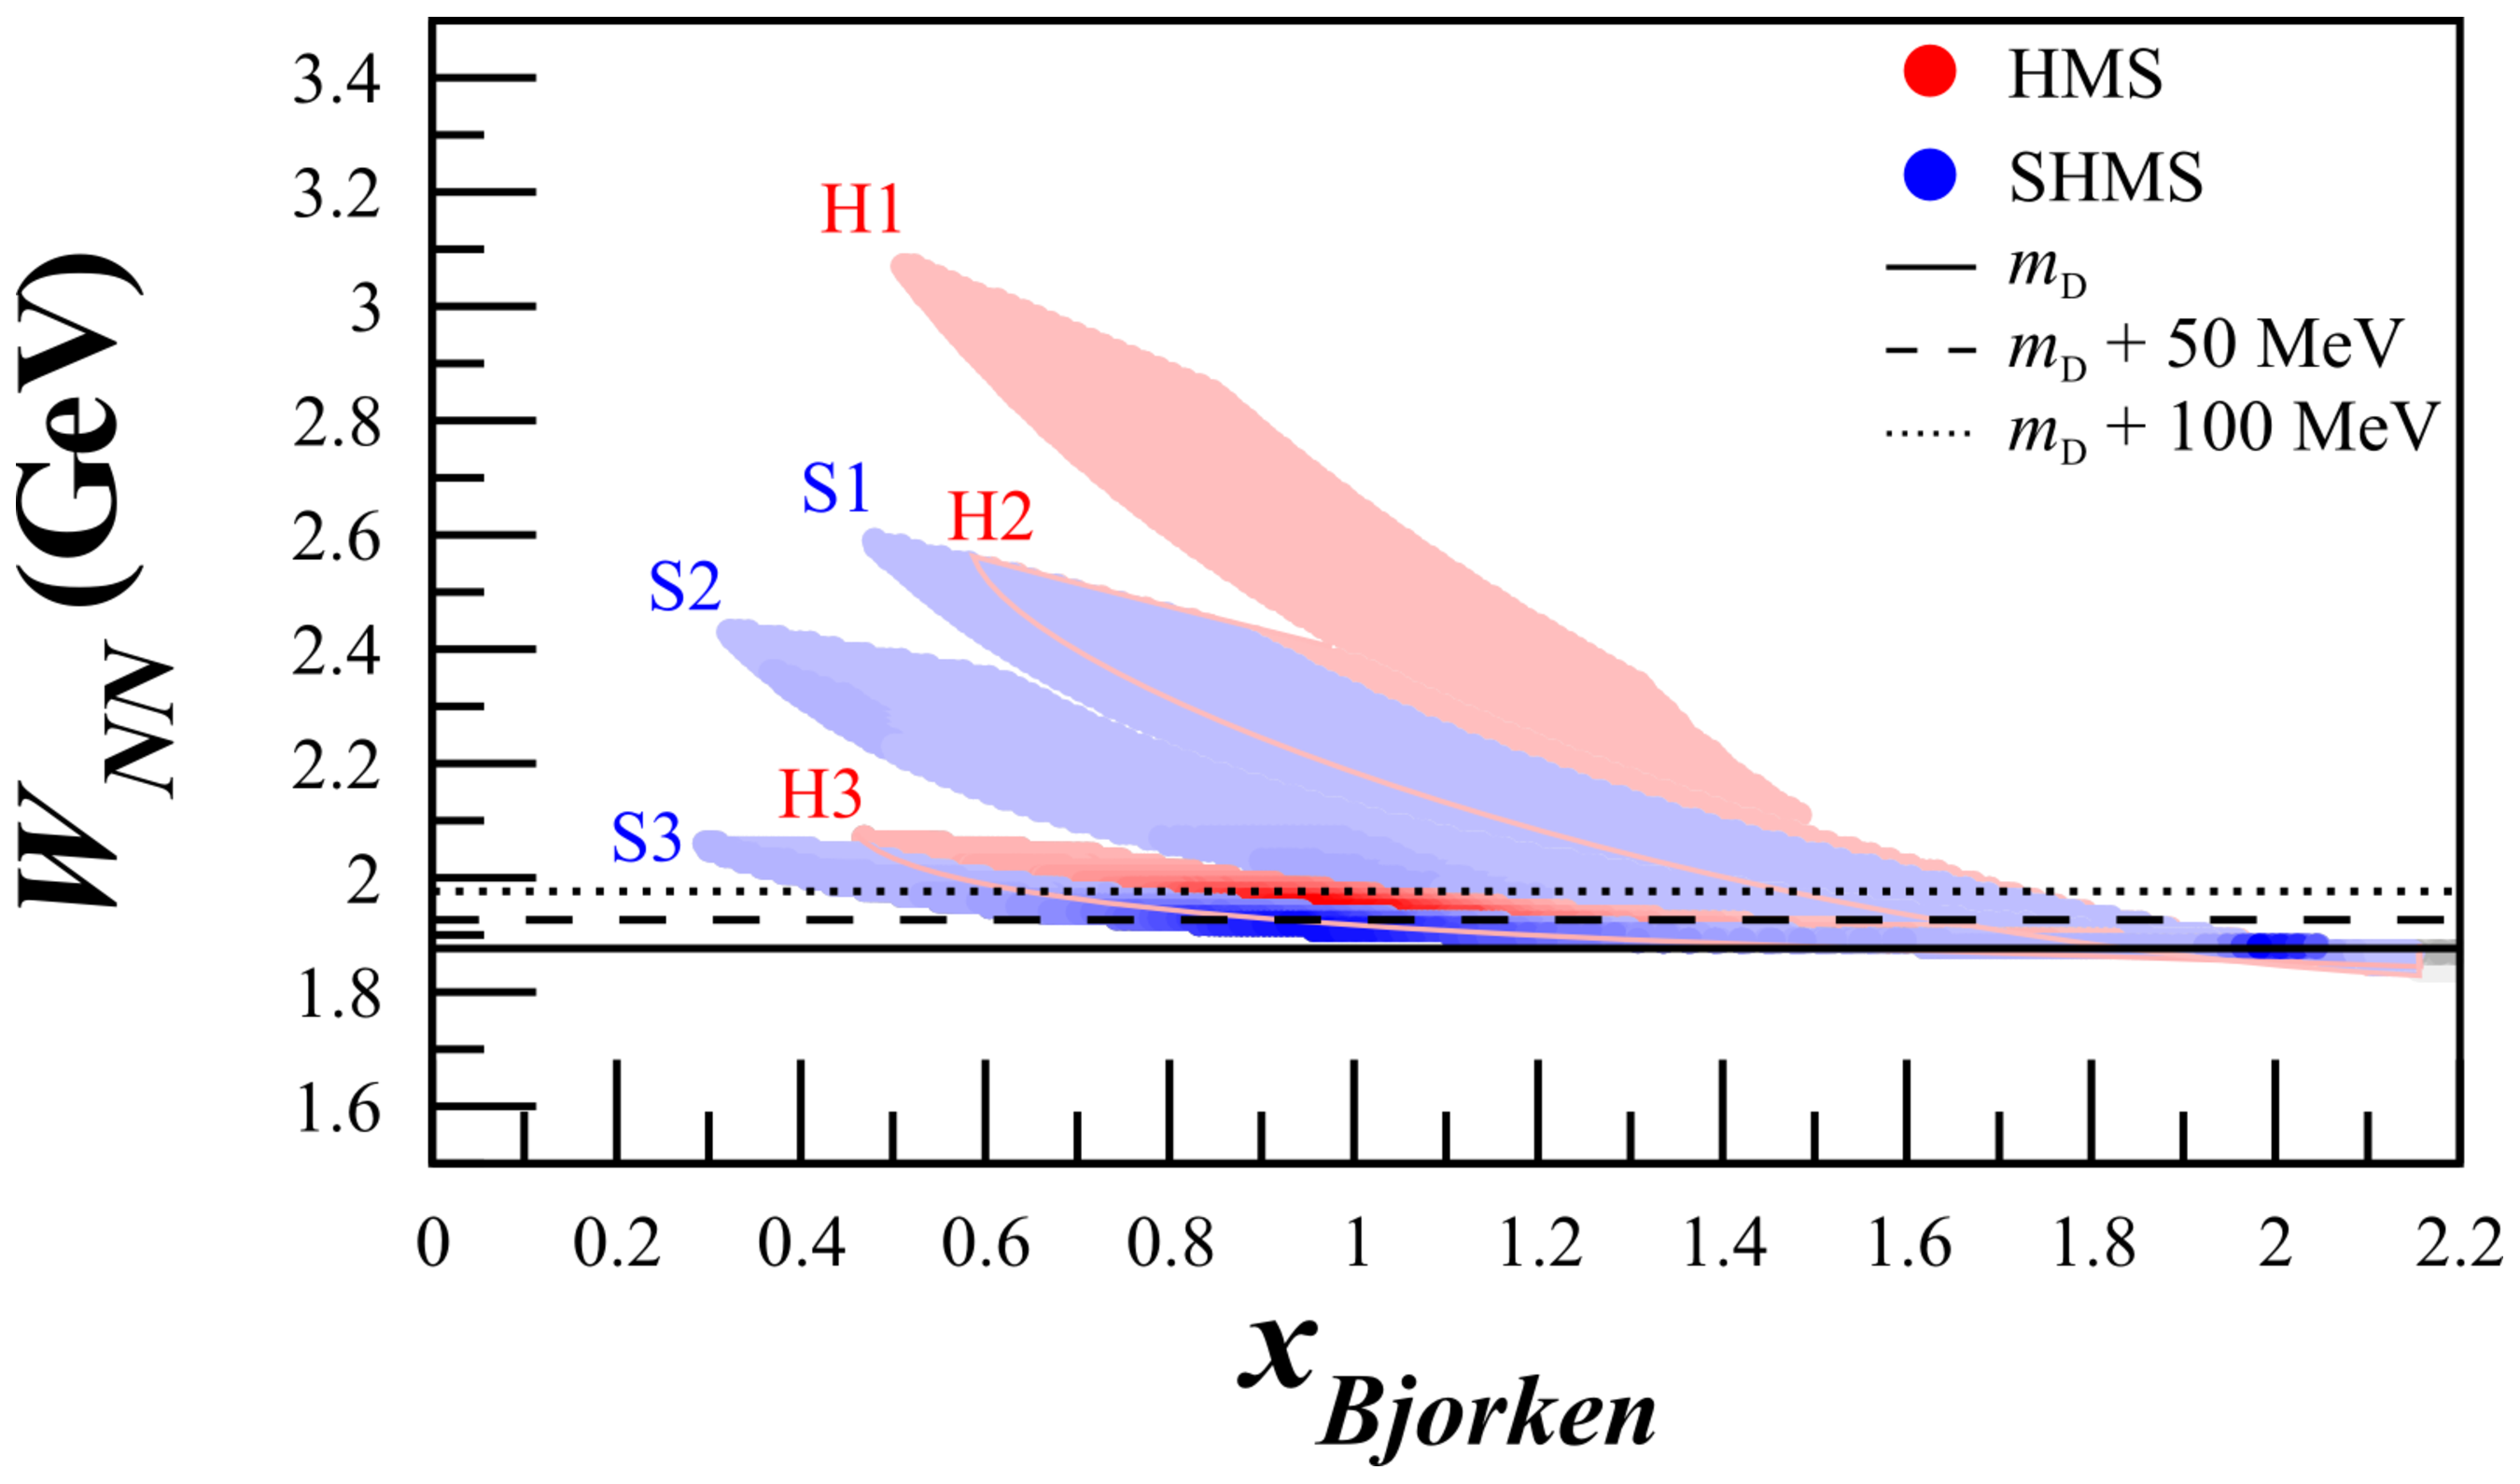
\includegraphics[width=0.49\textwidth]{figs/Pzz_30_all_wnn.eps} %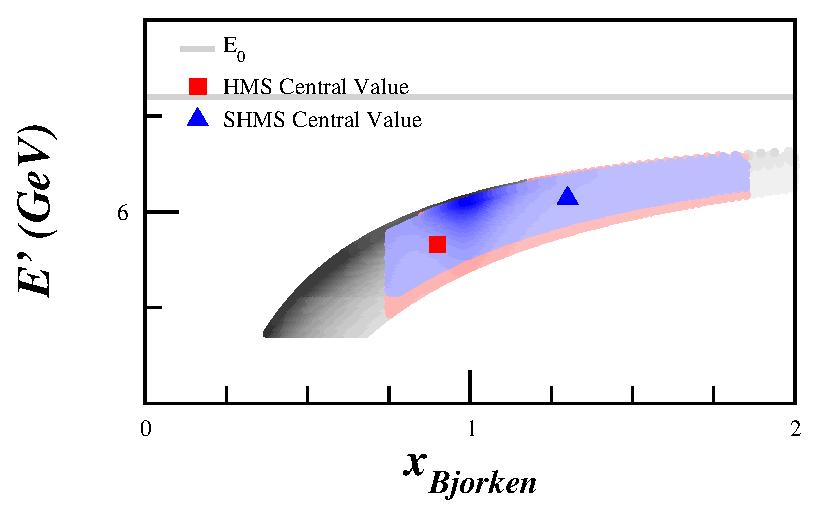
\includegraphics[width=0.49\textwidth]{figs/kine/Pzz_30_eprime.eps}
%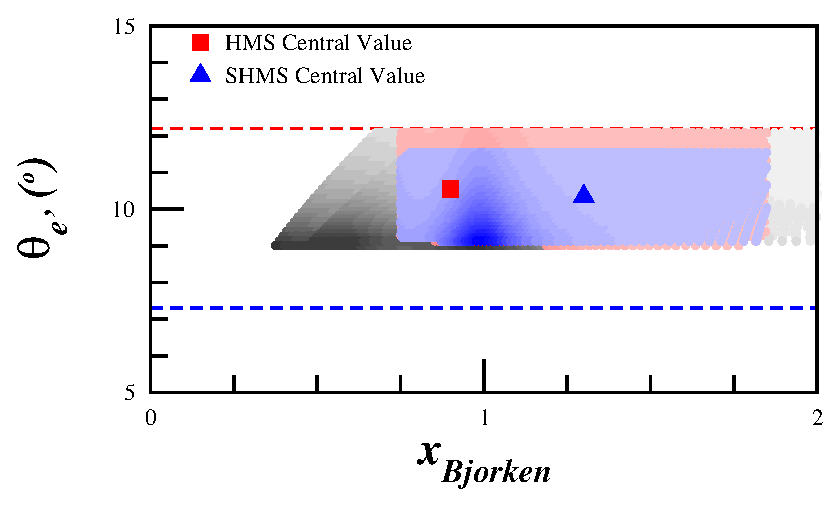
\includegraphics[width=0.49\textwidth]{figs/kine/Pzz_30_theta_eprime.eps}~~ 

\caption{\label{kincov-const} Kinematic coverage for the kinematics listed in Table~\ref{RATES1-const}, which can be achieved in the case that the SHMS is constrained to angles $>10^{\circ}$.}
\end{center}
\end{figure}



\begin{figure}
\begin{center}
\includegraphics[width=0.49\textwidth]{figs/Azz_shms_const.eps} \includegraphics[width=0.49\textwidth]{figs/t20_shms_const.eps} 
\caption{\label{PROJ-const}Projected uncertainties for the tensor asymmetry $A_{zz}$ and elastic analyzing power $T_{20}$ with \productiondays days of beam time using the constrained kinematics in Table~\ref{RATES1-const}.
}
\end{center}
\end{figure}
\fi

%\subsection{Overhead}

Table~\ref{OVERHEAD} summarizes the expected overhead, which sums to \overheaddays days.
%In order to calibrate the target polarimetry, elastic scattering measurements will be performed at %an
%incident energy of 2.2 GeV.
The dominant overhead comes from switching from the polarized to unpolarized state and vice versa, and target anneals.  The target will need to be annealed about every other day, and the material replaced once a week.
Measurements of the dilution from the unpolarized materials contained in the target, and of the packing fraction due to the granular composition of the target material will be performed with a carbon target.

%Configuration changes include rotation of the magnetic field of the target from parallel to perpendicular and vice versa.

\begin{table}
\begin{center}
  \begin{tabular}{lrrr} \hline\hline
 Overhead & Number&Time Per (hr)&(hr)\\
\hline
Polarization/depolarization & 35&       2.0&     70.0\\
Target anneal             &   13&       4.0&     52.0\\
Target T.E. measurement   &    5&       4.0&     20.0\\
%Beamline survey          &    2&       8.0&     16.0\\
Target material change    &    4&       4.0&     16.0\\
Packing Fraction/Dilution runs &    18&       1.0&      18.0\\
\hline
%Pass change              &    0&       4.0&       0.0\\
BCM calibration           &    8&       2.0&      16.0\\
Optics                    &    3&       4.0&      12.0\\
Linac change              &    1&       8.0&      8.0\\
Momentum/angle change     &    3&       2.0&       6.0\\
%Arc Energy Meas.          &    3&       2.0&       6.0\\
\hline
                          &     &          &        \overheaddays days  \\
\hline
 \end{tabular}
 \end{center}
  \caption{\label{OVERHEAD} Major contributions to the overhead.}
\end{table}


%\subsection{Polarized Target}
\label{POLTARGSEC}
This experiment will use the
JLab/UVa dynamically polarized solid {\TARGET}target operated in longitudinal mode.  
%Transverse polarization requires  operation of an upstream chicane to ensure proper transport through the target magnetic field.  
The target is typically operated with a specialized slow raster and beamline instrumentation capable of characterizing the low current 50-100 nA beam.
All of these requirements have been met previously in Hall C.
%, and will be soon implemented also in Hall A for the E08-027/E08-007 run in 2011. 
%
The polarized target (see Fig.~\ref{fig:target}), 
has been successfully used in experiments E143, E155, and E155x at SLAC, and E93-026, E01-006 and E07-003, E08-027 and E08-007 at JLab.
A similar target was used in Hall B for the EG1, EG4, and DVCS experiments. 
%although Hall B does
%not at present have the facilities necessary to operate a transversely polarized target with an electron beam.

The JLab/UVa target underwent significant renovation and improvement~\cite{CKEITH} during the recent g2p run. The magnet was replaced early in the run, and the target then performed consistently.   A new 1 K refrigerator and target insert were designed and constructed by the JLab target group.  The cryogenic pumping system has been overhauled.  In particular, the older Alcatel 2060H rotary vane pumps have been replaced with new Pfeiffer DU065 magnetically coupled rotary vane pumps, and the pump controls are being refurbished. The target motion system has been rebuilt from scratch. %And now, the magnet and vacuum jacket rotate independently of the refrigerator and target insert, which simplifies rotation from parallel to perpendicular magnetic field orientations.

%
\begin{figure}
\centering
\includegraphics[width=5.0in,clip]{figs/targnew.eps} %target_gimp.eps}
\caption{Cross section view of the JLab/UVa polarized target. The proposed experiment will use the modified Hall B magnet, where the backwards-scattering cone is blocked with quench protection circuitry. Figure courtesy of C. Keith.  \label{fig:target}}
\end{figure}


%\begin{figure}
%\centering
%\includegraphics[width=4.5in,clip]{figs/liD.eps}
%\caption{\label{fig:LID} Typical Deuteron thermal equilibrium (TE) and enhanced signals in $^6$LiD.  The left plot shows a typical deuteron TE and the right shows an enhanced deuteron NMR signal.  Note its clean undistorted shape unlike for $^{15}ND_3$.  Also, note the scale difference between the TE and enhanced signals.
%{\it Reproduced from Ref.~\cite{ALTOBIAS}}.}
%\end{figure}

\begin{figure}
\centering
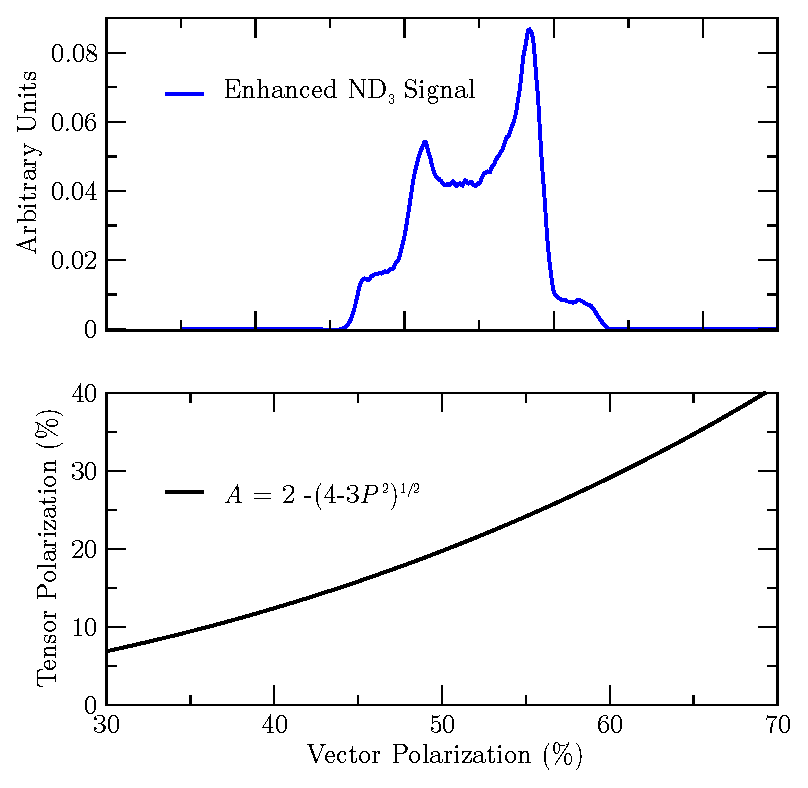
\includegraphics[width=0.5\textwidth]{figs/tensor_pol3.eps}
\caption{{\bf Top}: NMR signal for ND$_3$ with a vector polarization of approximately 50\% from the GEN experiment.  %The average polarization in beam for that experiment was 35\%. 
{\bf Bottom}: Relationship between vector and tensor polarization in equilibrium, and 
neglecting the small quadrupole interaction.  \label{fig:tensorpol}}
\end{figure}

%\begin{figure}
%\centering
%\includegraphics[width=3.0in,clip]{figs/gen.eps} %target_gimp.eps}
%\caption{Performance of the ND$_3$ target during the GEN experiment.  \label{fig:gen}}
%\end{figure}


The target operates on the principle of Dynamic Nuclear Polarization, to
enhance the low temperature (1 K), high magnetic field (5 T) polarization of solid
materials  by microwave pumping.
The polarized target assembly contains several target cells of 3.0 cm length
that can be  selected individually by remote control to be located in the uniform field
region of a superconducting Helmholtz pair. The permeable target cells are
immersed in a  vessel filled with liquid Helium and maintained at 1 K by use of a
high power evaporation refrigerator.
The coils have a 50$^\circ$ conical shaped aperture along the beam axis
which allow for unobstructed forward scattering.
%34$^\circ$ wedge shaped aperture along the vertically oriented midplane.

The target material is exposed to microwaves
to drive the hyperfine transition which  aligns the nucleon spins. 
 The heating of the target by the beam causes a drop of a few percent in
the polarization, and the polarization slowly decreases with time due to radiation
damage. Most of the radiation damage can be repaired by periodically annealing the target,
until the accumulated dose reached is greater than about 
%$ 17\times 10^{15}$ e$^-$/cm$^2$, 
 $0.5\times 10^{17}$~$e^-$/cm$^2$,
at
which time the target material needs to be replaced. 
%The luminosity of the polarized 
%material in the uniform field region is approximately $85\times 10^{33}$ cm$^{-2}$ Hz.

\subsubsection{Polarization Analysis} 
%Eq.~\ref{TENSORVECTOR} allows calculation of a target's tensor polarization once the vector polarization has been determined.  
The three Zeeman sublevels of the deuteron system ($m=-1,0,1$) are
shifted unevenly due to the quadrupole interaction~\cite{Meyer:1985dta}. This shift
depends on the angle between the magnetic field and the electrical field gradient, and gives rise to two separate transition
energies. Hence, the unique double peaked response displayed in Fig.~\ref{fig:tensorpol}.
When the system is at thermal equilibrium with the solid lattice, the deuteron polarization is known from:
\begin{eqnarray}
\label{VECT}
P_z = \frac{4+\tanh\frac{\mu B}{2 k T}} {3+\tanh^2\frac{\mu B}{2 k T}    }
\end{eqnarray}
where $\mu$ is the magnetic moment, and $k$ is Boltzmann's constant.  The vector polarization can be determined by comparing
the enhanced signal with that of the TE signal (which has known polarization).  This polarimetry method is typically reliable to about 3.9\% relative.

Similarly, the tensor polarization is given by: 
\begin{eqnarray}
\label{TENS}
P_{zz} = \frac{4+\tanh^2\frac{\mu B}{2 k T}} {3+\tanh^2\frac{\mu B}{2 k T}    }
\end{eqnarray}

From Eqs.~\ref{VECT} and~\ref{TENS}, we find:
\begin{eqnarray*}
\label{PZZEQN}
P_{zz}= 2 - \sqrt{4-3 P_z^2}
\end{eqnarray*}


In addition to the TE method, polarizations can be determined by analyzing NMR lineshapes as described in~\cite{Dulya:1997qc} with a typical  7\% relative uncertainty.  At high polarizations, the
intensities of the two transitions differ, and the NMR signal shows an asymmetry R in the
value of the two peaks, as shown in Fig.~\ref{fig:tensorpol}.  The vector polarization is then given by:
\begin{eqnarray}
\label{RVECT}
P_{z} = \frac{R^2-1}{R^2+R+1}
\end{eqnarray}
and the tensor polarization is given by:
\begin{eqnarray}
\label{TVECT}P_{zz} = \frac{R^2-2 R +1}{R^2+R+1}
\end{eqnarray}
This measuring technique can be used as a compliment to the TE method resulting in reduced uncertainty in polarization.


\subsubsection{Tensor Polarization Enhancement}
It is possible to enhance tensor polarization using RF irradiation on the oriented deuterium nuclei to manipulate the alignment.
Applying a saturating RF field on the pedestal of the smaller transition equalizes the substate $m=+1$ and $m=0$ populations
over 2/3 of the NMR signal.  This equalization over the range of a single pedestal leads to enhancement in tensor polarization with only a small loss
to the overall area ($\sim 2\%$).  Very recent studies at UVA using deuterated butanol have indicated that the tensor polarization can be increased by using a modified hole burning technique. The result will be investigated in the near future, and the method applied to ND$_3$.
% in a tensor polarization of more then25\% as shown in Fig.~\ref{fig:study}.  A similar result is expected for ND$_3$.  
The studies also indicate that microwaves used during DNP does not
interfere with the saturation from the RF irradiation when sufficient power is used.  This implies that RF over the pedestal can be done the same time DNP is performed to enhance the area while taking beam in an experiment.  Research and development is ongoing to study various
techniques to optimize tensor enhancement for nuclear experiments targets.
\begin{figure}
\centering
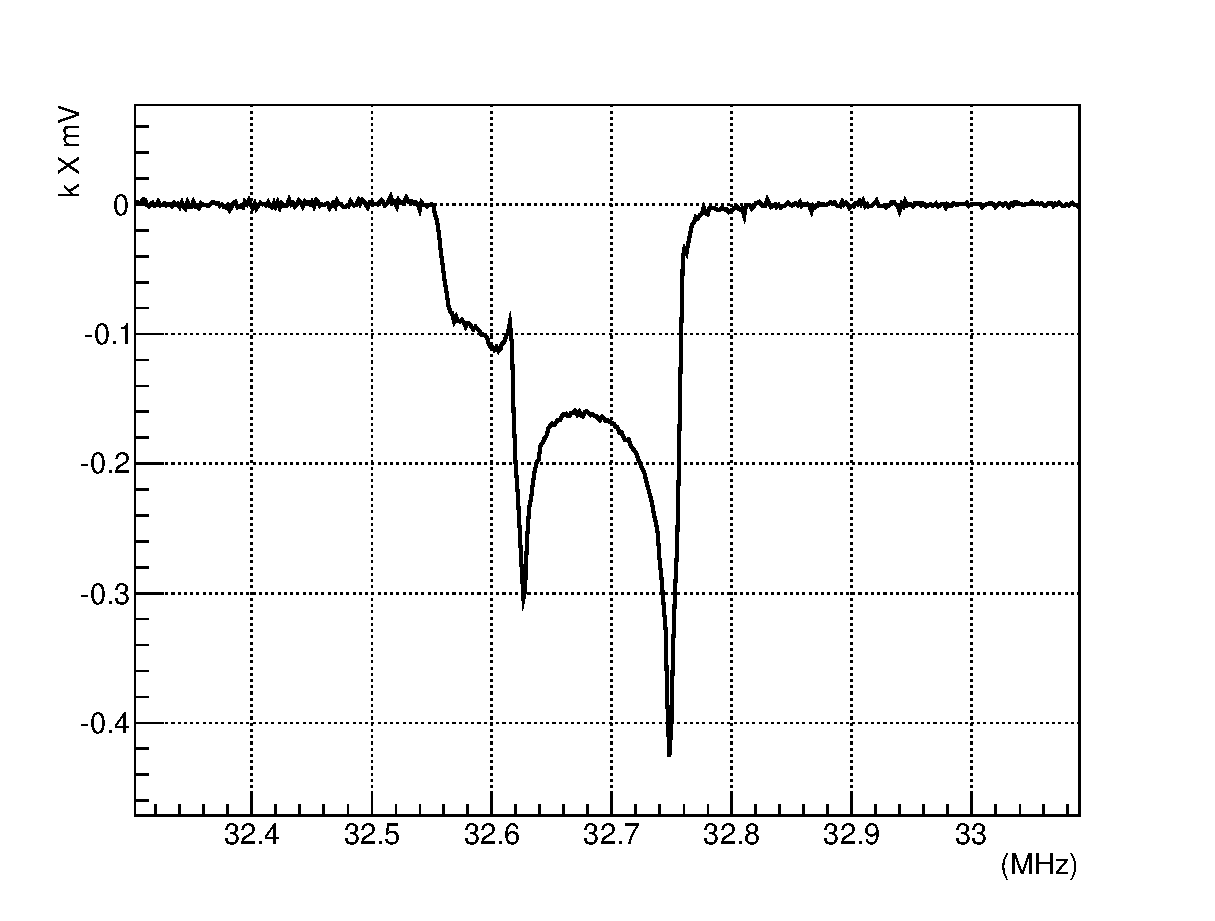
\includegraphics[width=3.0in,clip]{figs/study.eps}
\caption{The deuterium magnetic resonance line shape showing the recent achievement of 
%more than 25\%
high tensor polarization of deuterated butanol after RF saturation of a pedestal at the UVA polarized target lab accomplished during their April 2014 cool-down.}  
\label{fig:study}
\end{figure}

\subsubsection{Depolarizing the Target}
%The NMR will be used on both to probe polarization.  
To move from polarized to unpolarized measurements, the target
polarization will be annihilated using destructive NMR loop field changes and destructive DNP microwave pumping.
%It is also possible to remove LHe in the nose of the target to remove the polarization by heating.
During unpolarized data taking the incident electron beam heating is enough to remove the thermal equilibrium polarization.

We are able to verify that the target is in the unpolarized state via NMR measurements.  The target material will be
kept at 1 K for polarized and unpolarized data collection, and the target field
will be held constant for both states as well.  These
consistencies are used to minimize the systematic differences in the
polarized and unpolarized data collection.  To minimize systematic effects over
time, the polarization condition will be switched twice in a 72 hour period, as shown in Fig.~\ref{fig:polcycle}. 
This will be sufficient to account for drift in integrated charge accumulation.

\begin{figure}
\centering
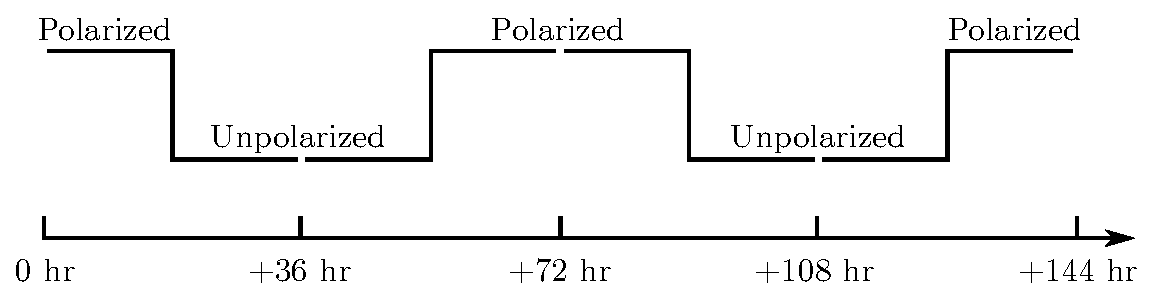
\includegraphics[width=0.75\textwidth,clip]{figs/pol_cycle.eps}
\caption{A visual demonstration of how the polarization cycle will happen over a 72 hour period to reduce time-dependent systematic effects. For the two lower $Q^2$ measurements, the cycle will happen over a 18 hour period.}  
\label{fig:polcycle}
\end{figure}

%(I think we should move this discussion to another section dealing with target
%physics and the overhead time accounting. Also,  I would favor dumping the LHe, and refilling the
%nose.)}


\subsubsection{Dilution Factor}
\label{dil}
To derive the dilution factor, we first start with the ratio of 
polarized to unpolarized counts.
%equation used to obtain the observable in terms of each measured cross section.
%\begin{equation}
%\frac{A_{zz}P_{zz}}{2}=\left(\frac{\sigma^1-\sigma}{\sigma}\right).
%\end{equation}
In each case, the number of counts that are actually measured,  neglecting 
the small contributions of the thin aluminium cup window materials, NMR coils, etc.,
are
\begin{equation}
N_1=Q_1\varepsilon_1 {\cal A}_1 l_1[(\sigma_N+3\sigma_1)p_f+\sigma_{He}(1-p_f)],
\end{equation}
and
\begin{equation}
N=Q\varepsilon {\cal A}l[(\sigma_N+3\sigma)p_f+\sigma_{He}(1-p_f)].
\end{equation}
where $Q$ represents accumulated charge, $\varepsilon$ is the dectector 
efficiency, ${\cal A}$ the cup acceptance, and $l$ the cup length.  

For
this calculation we assume similar charge accumulation such that $Q\simeq Q_1$, 
and that the efficiencies stay constant, in which case all factors drop out of 
the ratio leading to
\begin{eqnarray}
\nonumber \frac{N_1}{N}& = &\frac{{(\sigma_N+3\sigma_1)p_f+\sigma_{He}(1-p_f)}
}{(\sigma_N+3\sigma)p_f+\sigma_{He}(1-p_f)}\\
\nonumber & = & \frac{{(\sigma_N+3\sigma(1+A_{zz}P_{zz}/2))p_f+\sigma_{He}(1-p_
f)}}{(\sigma_N+3\sigma)p_f+\sigma_{He}(1-p_f)}\\
\nonumber & = & \frac{{[(\sigma_N+3\sigma)p_f+\sigma_{He}(1-p_
f)]+3\sigma A_{zz}P_{zz}/2}}{(\sigma_N+3\sigma)p_f+\sigma_{He}(1-p_f)}\\
\nonumber & = & 1 + \frac{3\sigma 
A_{zz}P_{zz}/2}{(\sigma_N+3\sigma)p_f+\sigma_{He}(1-p_f)}\\
& = & 1 + \frac{1}{2} f A_{zz}P_{zz}, 
\end{eqnarray}
where $\sigma_1 = \sigma(1+A_{zz}P_{zz}/2)$ has ben substituted, per 
Eq.~\ref{eq:one}, with $P_B =0$. It can be seen that the above result 
corresponds to Eq.~\ref{3}.



% \section{Summary}
%  
We request \production_days days of production beam time in order to  measure
the tensor asymmetry A$_{zz}$ and spin structure function $b_1$ using a 
longitudinally polarized deuteron 
%(\TARGET) 
target together with the Hall C HMS and SHMS spectrometers.
All existing theoretical predictions for $b_1$ in the region of interest predict small or vanishing
values for $b_1$  
%at intermediate values of $x$, 
in contrast to the apparent large negative result of the only existing measurement from HERMES. 
%Tensor structure measurements provide information not available from spin-1/2 targets. 

This experiment will provide access to the tensor quark polarization and allow a test of the
Close-Kumano sum rule, which vanishes in the absence of tensor polarization in the quark
sea.
Until now, tensor structure has been largely unexplored, so the study
of these quantities holds the potential of initiating a new field of spin physics at
Jefferson Lab.
%This measurement will help clarify the role quark orbital angular momentum plays in the nucleon spin, and open a new avenue of spin structure studies at Jefferson Lab.



\clearpage
\appendix
%\section{Rates and Kinematics}
%\begin{figure}
%\begin{center}
%\includegraphics[width=1.0\textwidth,angle=00]{newfigs/ellie/b1_rates_hms_shms.eps}
%\caption{\label{PROJDETAIL}
%{\bf Top Left: }
%Projected precision of the tensor structure function $b_1$  with \production_days days of beam time.
%{\bf Right:}
%Corresponding projected precision of the tensor asymmetry $A_{zz}$.
%Data at different $Q^2$ are combined with an x-binning that varies slightly per point, but is approximately $\pm0.05$.
%%The black band
%%represents the systematic uncertainty.
%Also shown are the HERMES data~\cite{Airapetian:2005cb}, and the calculations from Kumano~\cite{Kumano:2010vz}, Miller~\cite{Miller:1989nc,Miller_tmp}, and Sargsian~\cite{MISAK}.
%}
%\end{center}
%\end{figure}

%\section{Statistical error calculations of $A_{zz}$}
%\input{input/Azz_error.tex}
%\input{input/b1_error.tex}
%%\section{Statistical Uncertainty Calculation}
\label{stat}
To investigate the statistical uncertainty we start with the equation for $A_{zz}$ using
measured counts for polarized data $N_1$ and unpolarized data $N$, 
\begin{equation}
A_{zz}=\frac{2}{fP_{zz}}\left(\frac{N_1-N}{N}\right).
\end{equation}
The absolute error with respect to counts in then,
\begin{equation}
\delta A_{zz}=\frac{2}{fP_{zz}}\sqrt{\left(\frac{\delta N_1}{N}\right)^2+\left(\frac{N_1\delta N}{N^2}\right)^2}.
\end{equation}
To approximate, assume $N_1\simeq N$, so that twice $N$ is required to obtain the total number of count
$N_T$ for the experiment leading to,
\begin{equation}
\delta A_{zz}=\frac{4}{fP_{zz}}\frac{1}{\sqrt{N_T}}.
\end{equation}



%  Go to fullpage mode

\topmargin 0pt
\advance \topmargin by -\headheight
\advance \topmargin by -\headsep

\textheight 8.9in

\oddsidemargin 0pt
\evensidemargin \oddsidemargin
\marginparwidth 0.5in

\textwidth 6.5in
\clearpage
%\begin{thebibliography}{99}
%\input{input/bib.tex}
%\end{thebibliography}

\bibliography{input/bibliography}
\end{document}
